\documentclass[12pt]{report}
\usepackage[utf8]{inputenc}
\usepackage[a4paper, top=2.5cm, bottom=2.5cm, left=2.5cm, right=2.5cm]{geometry}
\usepackage[dvipsnames]{xcolor}
\usepackage{amsmath}
\usepackage{lipsum}
\usepackage{framed}
\usepackage{graphicx}
\usepackage{multirow}
\usepackage{wrapfig}
\usepackage{bbold}
\usepackage{afterpage}
\usepackage{subcaption}
\usepackage{float}
\graphicspath{{Images/}}
\usepackage{algorithm}
\usepackage{algpseudocode}
\renewcommand{\algorithmicrequire}{\textbf{Input:}}
\renewcommand{\algorithmicensure}{\textbf{Output:}}


\algnewcommand\And{\textbf{and }}
\algnewcommand\Or{\textbf{or }}
\usepackage{fancyhdr}
\DeclareMathOperator*{\argmax}{arg\,max}
\DeclareMathOperator*{\argmin}{arg\,min}


\pagestyle{fancy}
\begin{document}

\definecolor{light-gray}{gray}{0.87}  

\begin{titlepage}
\hspace*{-3.5cm}
    \begin{minipage}{\textwidth}
        \vspace{-2.5cm}
        \begin{center}
    

            
\includegraphics[width=\paperwidth]{LogoEHU.PNG}
        \end{center}
    \end{minipage}

\vspace{1cm}

\hspace{-3.1cm}
\noindent\fcolorbox {light-gray}{white}{

    \parbox{\paperwidth}{
     \begin{center}
     \large Final Degree Project
    \\
             \large Physics Degree

\end{center}
    }
    }


\vspace{0.8cm}

\noindent\hspace*{-2.5cm}%
\colorbox{light-gray}{\begin{minipage}{\paperwidth}%

    \vspace{1cm}

    \color{RoyalBlue}
    \centering\Large\textbf{ Activity Prediction for Intermediate Conductance\\ Calcium-Activated Potassium Channel Inhibitors\\ using Random Forest}



    \vspace{7cm}\mbox{}
  \end{minipage}
}

\begin{flushright}
 Author:
\\
Christian Dorado Cerrato
\\
 Directors:
\\
Aitor Bergara Jauregui
\\
Aritz Leonardo Liceranzu

\end{flushright}

\begin{center}
\noindent\fcolorbox {white}{white}{

    \parbox{11cm}{
         \begin{center}
    \footnotesize © 2022, Christian Dorado 
    \\
   \small http://es.creativecommons.org/blog/licencias/

        \end{center}
    }
    }
\end{center}

\hspace{-3.2cm}
\noindent\fcolorbox {light-gray}{white}{
    \begin{minipage}[]{1000pt}

        \parbox{\paperwidth}{
            \begin{center}
    
                 Leioa, $4^{th}$ October 2022

            \end{center}
        }
    \end{minipage}
}
\end{titlepage}


%%%%%%%%%%%%%%%%%%%%%%%%%%%%%%%
%Hemendik aurrera hasi lana idazten%
%%%%%%%%%%%%%%%%%%%%%%%%%%%
\begin{abstract}
\begin{center}
Ion channels, located in the membrane of cells, are a great deal when referring to regulation of ion transport in our body. Potassium channel inhibitors play a grand role in the regulation and so-called intermediate conductance of this well-known and mapped channel called SK4. Using machine learning techniques, the inhibitory capacity of any molecule can be addressed by approximation, giving very good results and not having to wait for yearlong biological simulations. This allows to target potentially functional drugs much faster and easier, without that much computer and time expense.
\end{center}
\vspace{10cm}
Another approach can be given. After the ``Introduction" section, you may begin to explore the procedure in the ``Application" section and return to the ``Machine Learning" section if needed to better understand the concepts used.



\end{abstract}
\tableofcontents

\chapter{Introduction}
\hspace{1.5cm}Potassium ion channels are membrane proteins critically involved in the regulation of fundamental physiological processes such as cell volume, membrane potential, and hormone secretion. To allow for the tuning of these processes, the human genome contains 78 potassium channels. The small- and intermediate conductance calcium-activated potassium channels are a group of proteins within the overall potassium channel family that share a set of common features.

One of their main features is that they are considered calcium-activated channels because their gating mechanism, in which potassium flux is regulated by the opening and closing of the channel, is modulated by a calcium-sensing protein called calmodulin.

\begin{figure}[h]
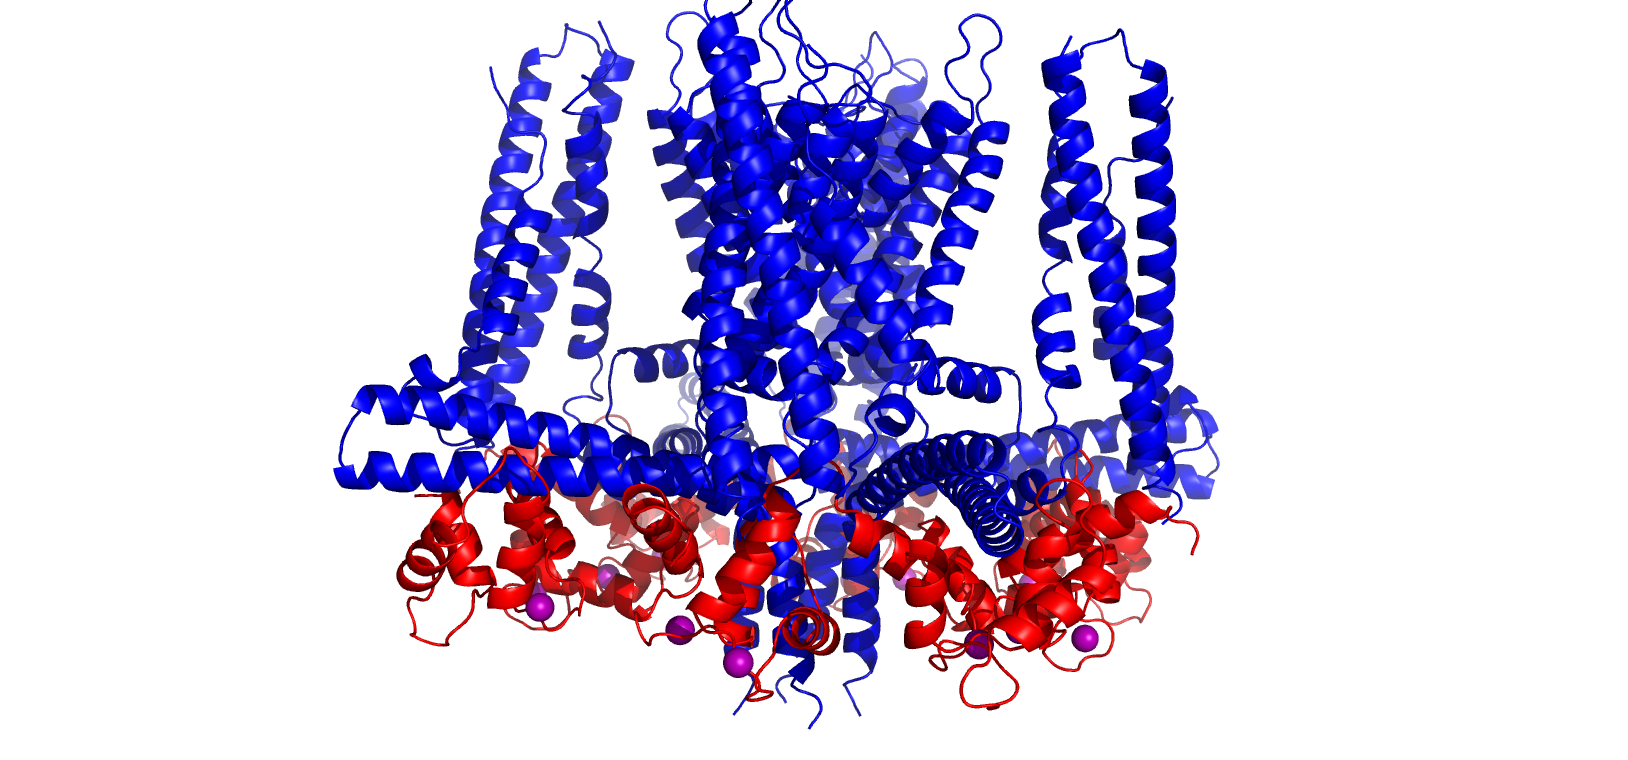
\includegraphics[width=15cm, height=7.5cm]{Images/Introduction/sk4.png}
\centering
\caption{Illustration of the $\text{K}_{\text{Ca}}3.1$ channel, based on the experimentally solved structure in \cite{sk4_struct}.}
\label{fig:Figure 3.1}
\end{figure}

In addition, small and intermediate conductance channels are so called because of their small single channel conductance in the order of 10 pS, in contrast with large conductance channels which have very high conductance in the range of 100 to 300 pS.

The protein studied in this study is the $\text{K}_{\text{Ca}}3.1$, and is a member of the small and intermediate conductance calcium-activated potassium channel subfamily, and is mainly expressed in red blood cells and cells of the immune system. Their structure, which was recently solved by MacKinnon \textit{et al.} \cite{sk4_struct} and is shown in Figure 1.1, is tetrameric, that is, it consists of four identical subunits. Each of these subunits contains six domains that insert into the cell membrane and form the potassium ion selectivity filter. In addition, the channel contains a calmodulin-binding domain inside the cell, where calcium-sensing calmodulin binds to the protein.  An schematic illustration of this structure is shown in Figure 1.2.

\begin{figure}[h]
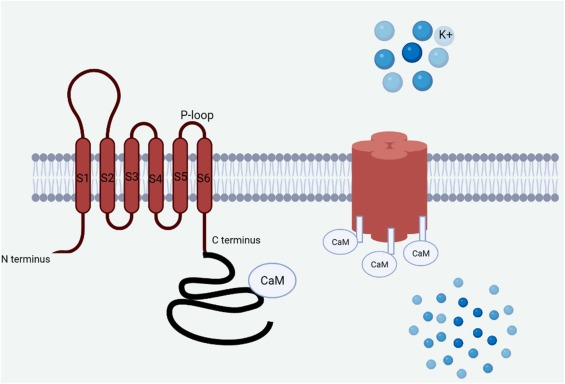
\includegraphics[width=12cm, height=7.5cm]{Images/Introduction/SK_Channel_schema.jpg}
\centering
\caption{General small and intermediate conductance channel structure. Four subunits form the channel complex (right). Each alpha subunit consists of 6 transmembrane domains (S1-S6) (left). Note N and C termini, with a calmodulin (CaM) binding domain at the C terminus of each subunit. Image from \cite{sk4_schema}.}
\label{fig:Figure 3.1}
\end{figure}

The main reason why this channel is interesting to us is that it has been validated as a potentially interesting pharmaceutical target. It has been shown that small molecule inhibitors of this channel may be used for the treatment of diseases such as vascular restenosis \cite{vascular_restenosis}, atherosclerosis \cite{atherosclerosis}, allograft vasculopathy \cite{allograft_vasculopathy}, inflammatory bowel disease \cite{inflammatory_bowel_disease}, ischemic stroke \cite{ischemic_stroke}, and renal \cite{renal_fibrosis} and cardiac fibrosis \cite{cardiac_fibrosis}. The action mechanism of one of these inhibitors is shown in Figure 1.3, where it can be seen that the inhibitor lies in the middle of the channel gate blocking the flow of potassium in and out of the channel and thus reducing its conductance.

Despite their potential application, no small molecule $\text{K}_{\text{Ca}}3.1$ channel inhibitors that are suitable for clinical use are known yet, due to different pharmacological issues with the currently known inhibitors. This serves as the main motivation for this work, where we are interested in analysing whether computation techniques based on machine learning can serve as useful aids in the search of clinically viable $\text{K}_{\text{Ca}}3.1$ channel inhibitors.

\begin{figure}[h]
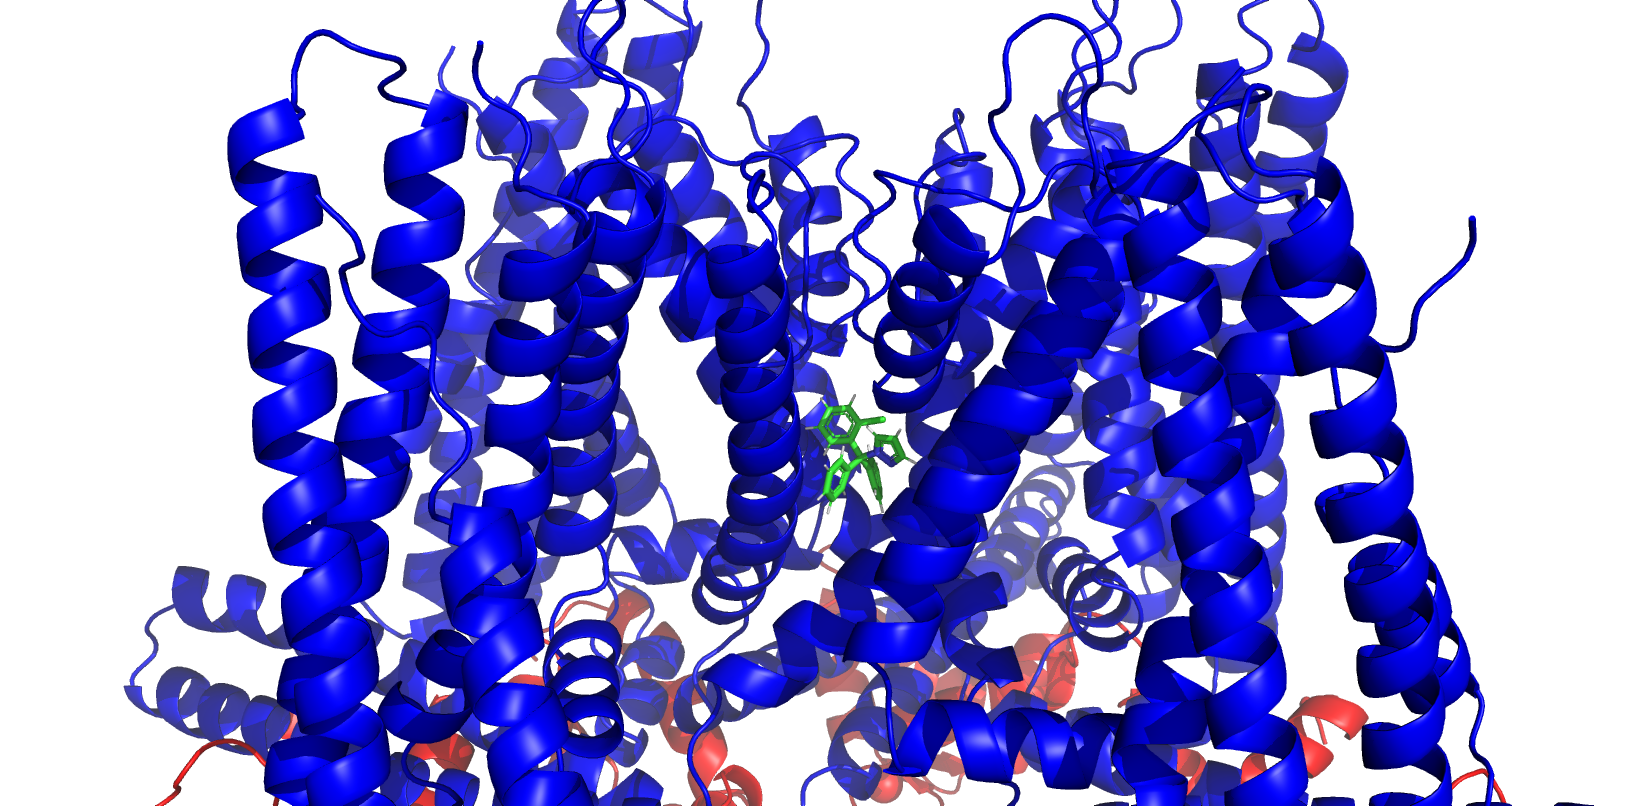
\includegraphics[width=12cm, height=7.5cm]{Images/Introduction/tram34_docking.png}
\centering
\caption{Bound conformation of the TRAM-34 ligand in the binding pocket of the $\text{K}_{\text{Ca}}3.1$ channel that lies at its gate. TRAM-34 is a distinguished and potent inhibitor of intermediate conductance in calcium-activated potassium channels.}
\label{fig:Figure 3.1}
\end{figure}

In recent years, as traditional experimental techniques for the discovery of new drugs have gradually become more expensive and less effective, computational techniques have become significantly more relevant in the field of drug development.

One of the most common computational techniques for drug development is molecular docking, which is used to predict the binding of small molecules (also referred to as ligands in this context) to a target protein of interest (also referred to as a receptor in this context). While these techniques have become quite accurate in predicting the geometric conformations that these ligands adopt when binding to most systems, they are much less effective in predicting the binding affinity between the ligands and the receptor. The binding affinity indicates how favourable the binding is between the ligand and the receptor, and can be understood as the difference in free energy between the bound and unbound systems.

This measure is extremely important for drug discovery because it can be used to distinguish nonbinding ligands and to identify binders in large compound libraries with a very large number of molecules. It is also used in the context of lead optimisation, where the goal is usually to identify the most effective molecules among those that have a similar chemical structure to a lead.

To predict this binding affinity, docking algorithms use $scoring$ $functions$ with a predetermined functional form inspired by theory for the relationship between the features that characterize the protein-ligand complex and its predicted binding affinity. It is almost always assumed that this relationship is linear. However, many complexes do not conform to this strong modeling assumption, and in these cases less accurate predictions are obtained.

Because of these limitations, there has been recent interest in using data-driven machine learning strategies to predict binding affinities between ligands and receptors. Machine learning algorithms are able to circumvent the constraint of a fixed functional form for the scoring function and can therefore implicitly capture intermolecular binding interactions that are difficult to model explicitly.\\

With this in mind, the main goal of this work is to investigate whether we are able to use machine learning strategies to improve the performance of conventional scoring functions, and thus serve as a potential contribution to future studies aimed at finding inhibitors that are clinically useful. Therefore, our strategy will be to use the docking simulations to predict the binding conformation of the inhibitors of the $\text{K}_{\text{Ca}}3.1$ channel, and then based on features of this conformation, along with features inherent to the chemical structure of the ligands, develop an algorithm that accurately predicts the binding affinity between the ligand and the receptor.

\chapter{Machine Learning}

\hspace{1.5cm}2021 marked the 80th anniversary of the invention of modern computer technology, an industry that has grown exponentially since then and has been a great help. Certainly, the human brain also has its limits, yet many try to understand things that cannot be achieved with conventional thinking. Sometimes it is even impossible to understand what lies behind a complex process, but as with the invention of computer technology, machine learning opens a multitude of doors that need to be opened, not understood.\\ 


\section{Introduction to Machine Learning}
Machine learning (ML) is nothing but a powerful tool with an unimaginable range of applications. Not only is it used in everyday life for seemingly difficult tasks, but every day new applications are found and explored that are enormous. In this case, despite the tremendous advances in software optimisation, simulating a complex biological environment is a difficult and, more importantly, expensive task that still has a ways to go. These types of problems are the focus of machine learning because it uses an alternative approach. Instead of tackling  the problem in the profound sense, ML aims to collect data and fill in the gaps to optimise the prediction error. This is very useful because the underlying understanding of the process is not required for the prediction to turn out pretty well, and in many cases, better. This is fascinating. As mentioned earlier, the main role of ML is to optimise problems, but for this to happen, some conditions must be met.\\

We humans need some kind of experience to learn, and patterns are used to build behaviours that we think are best for the situation onward.
Machine learning is somehow similar, a \textbf{dataset}, which would be analogous to experience, consists of \textbf{features} or attributes of each situation. There are two types of features:
\begin{itemize}
    \item \textbf{Response features}  are the features for which we want the model make predictions. For this to happen, some other features' information which may give us hints on how to solve the problem is required. These features need to be linked to the response features somehow, and hand out valuable information.
    
    
    \item \textbf{Descriptors} are the kind of features which set up the context surrounding the response features. Therefore, they need to have to do with the response features. The better the link between descriptors and response features, the better the prediction.

\end{itemize}
\vspace{0.6cm}

Using these attributes, algorithms can be trained minimising the error between the response variable estimations and the actual observations. They can shape models which best adequate to every possible situation; the bigger the dataset and the more the information in the features, the more accurate the model built by the algorithm. Algorithms themselves are optimisable functions with their own \textbf{hyperparameters} that can be tuned according to the context. There are many times of algorithms, from \textbf{regressors}, algorithms for which the response variable is continuous; \textbf{classifiers}, for which the response feature is discrete; to \textbf{clustering algorithms}, which do not need a response variable.\\

Regressors and classifiers can also be more simple or more complex; algorithms which build linear model are considered the most simple, while non linear model building algorithms or even ensemble methods (methods which use up more than one algorithm at once) are considered more complex. Sometimes, a simple one is enough to build a reliable model; in this case, it will be demonstrated a complex one better approximates to the situation of this burdensome biological problem.

\section{Machine Learning Algorithms}
To better understand the world of machine learning, we need to describe the underlying algorithms, and a few examples will make it clearer how it works.
\subsection{Linear Regression}
Among the algorithms of ML, the linear regression algorithm is the simplest of all and the easiest to understand. 
A linear regression algorithm aims to learn a function that makes predictions for the response variable by a linear combination of the input variables (or descriptors) \cite{Zhou21a}, that is, having an input vector $X=(x_1,x_2,x_3,...,x_M)$ corresponding to the $M$ descriptor features, the form of the estimation is:
\begin{equation}
\label{eqn:f(X)}
    f(X)=\beta_0+\sum_{i=1}^M\beta_ix_i,
\end{equation}
where $\beta=(\beta_0,\beta_1,...,\beta_M)$ are the coefficients linked to $(1,X)$, and $f(X)$, the response variable estimation.

To calculate the optimal coefficients that best predict the outcome, the $least$ $squares$ method is usually used. Here, the residual sum of squares (RSS) is defined as the loss (or cost) function, $i.e.$, the function to be minimised:
\begin{equation}
\label{eqn:RSS}
RSS(\beta)=\sum_{i=1}^N(y_i-\hat{y}_i)^2.
\end{equation}
where N is the number of observations; $\hat{y_i}$ is the estimate of each observation, or put another way, $\hat{y_i}=f(\textbf{X}_i)$, where \textbf{X} is the N x M matrix of descriptors/observations corresponding to the dataset; and $y_i$ is the actual value of the response feature for each observation column $\textbf{X}_i$.

After a little algebra (attached demonstration in appendix), the $\beta$ that best fits the model is as follows:
\begin{equation}
    \beta=(\textbf{X}^T\textbf{X})^{-1}\textbf{X}^T\textbf{y}
\end{equation}
where $\textbf{y}=(y_1,y_2,...,y_N)$. Then $f(X)$ can be properly addressed using equation \ref{eqn:f(X)}.
 
\subsubsection{Ridge}
In ridge regression, a regularisation parameter\footnote{A regularisation parameter is usually used to avoid overfitting the model. By setting the RSS with this regularisation parameter, the coefficients in the variables are penalised, so there is a chance to make a leaner or tighter prediction depending on whether the model is sufficiently constrained on the training data and whether it performs well on the raw data.} is attached to the previous RSS, which is minimised. As a result, the new RSS looks like this:
\begin{equation}
    RSS(\beta_{ridge})=\sum_{i=1}^N(y_i-\hat{y}_i)^2+\alpha \sum_{i=1}^M\beta_i^2,
\end{equation}
where $\alpha(>0)$ is a tuning parameter, so it can be changed to get a better prediction.

This linear regressor is a better option as it adapts to the context and the problem better and is a choice which (when $\alpha$=0) can implement  the simple linear regression explained earlier.\\

Ridge regression is defined in the procedure below:

\begin{algorithm}[H]
\caption{Ridge Regression}
\begin{algorithmic}[1]
    \Require Training set $D = \{ (\textbf{X}_1, y_1), (\textbf{X}_2, y_2), . . . , (\textbf{X}_N, y_N)\}$;
    
    Regularisation parameter $\alpha$.
    \Ensure $f(X)$ regression function.
    
    \For{$i \gets 1$ to $N$}
    \State Define $\hat{y}_i$: \begin{equation}
        \hat{y}_i=f(\textbf{X}_i)=\beta_0+\sum_{i=1}^M\beta_i\textbf{X}_i
    \end{equation}
    
    \EndFor
    \State Find the new $\beta_{ridge}=(\textbf{X}^T\textbf{X} + \alpha \mathbb{1})^{-1}\textbf{X}^T\textbf{y}$ (demonstration in appendix) or: \begin{equation}
        \argmin_{\beta}\sum_{i=1}^N(y_i-\hat{y}_i)^2+\alpha \sum_{i=1}^M\beta_i^2
    \end{equation}
    \State Tune $\alpha$ for optimal results.
\end{algorithmic}
\end{algorithm}
\subsection{Tree-Based Methods}
Although linear regression may seem as a powerful candidate, when it comes to describing such complex processes as the changes in conformations in proteins, it will be demonstrated more complex yet more computationally expensive methods are needed. For this, Random Forest is huge candidate. Random Forest is a nonlinear ensemble algorithm from the family of tree-based methods that implements the decision tree algorithm multiple times (hence the Forest designation). It has proven to be a viable candidate in many biological problems such as gene expression \cite{geneexpression} and damage localisation \cite{DNAdamage}, protein ligand residue recognising \cite{bindingresidues} or even closer, for many protein structure prediction techniques \cite{KALAISELVI2020107885}.

Lets firstly start by defining the components of this Random Forest algorithm, decision trees.
\subsubsection{Decision Trees}
Decision trees build regression (or classification) models using a tree structure. The dataset is optimally partitioned among features so that a decision can be made. Each of these resting datasets is called a node, and they represent the different levels of this decision tree. A representative illustration of a decision tree is Figure 2.1, which can serve as a guide.\\

A root node containing all the data used in training the algorithm optimally splits into two datasets (parent node splits into two child nodes) according to a single feature. For this optimal split, the $squared$ $error$ criterion was used, looking for the split with the smallest mean squared error (Section 2.4.1). After each split, either a terminal node or a decision node can be the new node. Decision nodes are those that can be split further, while end nodes are those that are not able to further split. There are several ways to determine whether a node will be a decision or terminal node: the number of observations in the node, the layer of the algorithm (the maximum depth hyperparameter can be set), the variance in the node...\\\\

\begin{figure}[h!]
    \centering
    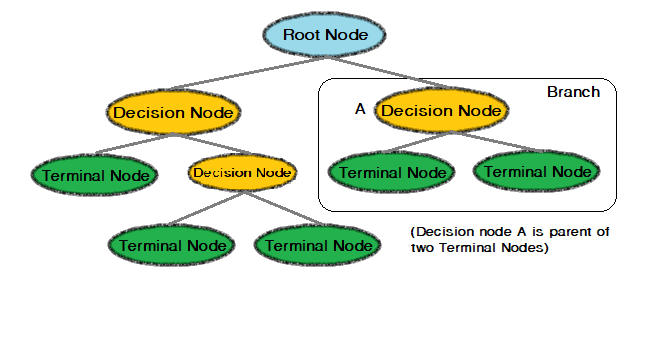
\includegraphics[width=0.85\textwidth]{Images/Methods/detreenodes.png}
    \caption{Visual Representation of a Decision Tree.}
\end{figure}
Each terminal node is assigned a response feature value, which is the mean value of the response feature of all observations in that cluster. The goal of decision trees, as with any regressor, is to predict the response feature value for new data containing descriptor information. After the new data point has passed through the decision trees, it is assigned the response feature value of the terminal node at which it arrived.\\\\ 
The algorithm for decision tree learning is on the next page.
\begin{algorithm}[H]
\caption{Decision Tree Learning}
\begin{algorithmic}[1]
    \Require Training set $D = \{ (\textbf{X}_1, y_1), (\textbf{X}_2, y_2), . . . , (\textbf{X}_M, y_M)\}$;
    
    Feature set $A = \{a_1, a_2,..., a_N\}$.
    
    
    
    \Ensure A decision tree with root node $i$.
    
    \hspace{-1.5cm}\textbf{Process:} Function Tree($D, A$)
    
    \State Generate node $i$.
    \If {All samples in $D$ belong to the same class $C$}
    
    \State Mark node $i$ as a class $C$ terminal node; {\Return}
    \EndIf
    \If {$A =\{\emptyset\}$ \Or all samples in $D$ take the same value on $A$}
    
    \State Mark node $i$ as a terminal node, and its class label is the majority 
    
    class in $D_i$; {\Return}
    \EndIf
    
    \State Select the optimal splitting feature $a_*$ from $A$
    
    \For{each value $a_*^\nu$ in $a_*$}
    
    \State Generate a branch for node $i$; Let $D_v$ be the subset of samples
    
    taking value $a_*^v$ on $a_*$;
    
    \If{$D_\nu$ is empty} 
    
    \State Mark this child node as a terminal node, and label it with the 
    
    \hspace{0.65cm}majority class in $D$; {\Return}
    \Else
    
    \State Use Tree($D_v , A \backslash \{a_*\}$) as the child node.
    
    \EndIf
    \EndFor
    
\end{algorithmic}
\end{algorithm}
\hspace{14cm}\cite{Zhou21a}\\






\subsubsection{Random Forest}
Random Forest (RF) is a decision tree founded algorithm whose idea is to merge various trees
through the idea of ensemble learning. There is no union linking each decision tree, but each and every decision tree in the forest shape the
final product (or output) of this model. 
In a regression problem, the average output of the individual decision trees is the final result \cite{YUAN2022100026}.\\

The feature sample for the decision trees in the Random Forest is chosen arbitrarily, they sample without replacement. This means, when a set of features needs to be determined for each decision tree, this is carried out randomly, and as well as more than one decision tree being able to contain the same feature, the same feature can appear twice in each decision tree (bootstrapping in Section 2.5.3).\\

As it can be observed in Figure 2.2, each decision tree is usually different, as it consists of distinct feature organisations, and as the input travels through each decision tree, it gets a response feature value. All this values are merged in a mean to get the final output. 
\begin{figure}[h!]
    \centering
    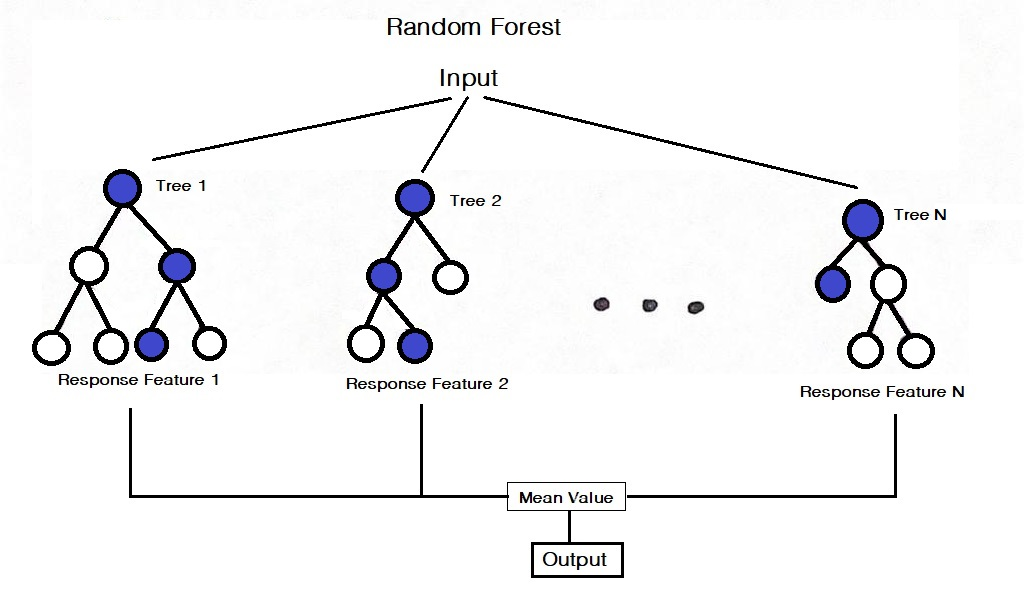
\includegraphics[width=0.8\textwidth]{Images/Methods/RFout.jpeg}
    \caption{A Random Forest simplified diagram. The input descriptor data travels through N decision trees where the blue nodes represent the decisions taken in every split. The mean is taken of every response feature value.}
\end{figure} 
\subsection{Clustering Algorithms}
When talking about machine learning algorithms, clustering algorithms are a big part of what is called $unsupervised$ $learning$ in the machine learning culture. These algorithms, as the name itself remarks, do not require tags or response variables of any sort, as they are programmed to find patterns in the raw data. Clustering algorithms classify the data into different groups, taking into account similarities, and they can be very useful in sorting molecules or even descriptors themselves by taking into account the correlation between them.

\subsubsection{K-means Clustering}

K-means is a widely known clustering method, the simplest and in many cases the most useful. In k-means, n observations are clustered into a number of k clusters. The criterion used to determine whether an observation belongs to one cluster or another is the minimum distance\footnote{The distance described in these clustering algorithms refers to the p-dimensional euclidean distance in the descriptor space. For example, the distance between two observations a and b with 4 descriptors each $(x_1,x_2,x_3,x_4)$ is determined by:
\begin{equation}
    d(a,b)=\sqrt{\Delta x_1^2+\Delta x_2^2 + \Delta x_3^2 + \Delta x_4^2}
\end{equation}
where \Delta x_i=x_{ia}-x_{ib}.} to the mean of the descriptors of all the observations in every cluster, also known as the centroid.\\

The k-means algorithm works upon two principal steps, assignment and updating, which are iterated until convergence, when further iterations do not change the outcome of each and every cluster.\\\\

\begin{figure}[H]
    \centering
    \begin{subfigure}[H]{0.2\textwidth}
        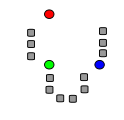
\includegraphics[width=\textwidth]{Images/Methods/K-means/K_Means_Example_Step_1.png}
        \vspace{-20pt}
        \caption{To initialise k-means, k (k=3 in this case) different cluster centroid points need to be randomly set.}
    \end{subfigure}
    \quad
    \begin{subfigure}[H]{0.2\textwidth}
        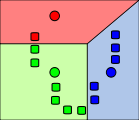
\includegraphics[width=\textwidth]{Images/Methods/K-means/K_Means_Example_Step_2.png}
        \vspace{1pt}
        \caption{Then, the observations need to be assigned to the cluster whose centroid is closer to it, therefore the $assignment$ $step$.}
    \end{subfigure}
    \quad
    \begin{subfigure}[H]{0.2\textwidth}
        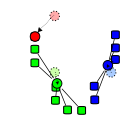
\includegraphics[width=\textwidth]{Images/Methods/K-means/K_Means_Example_Step_3.png}
        \vspace{-10pt}
        \caption{After the assignment is done, the mean of the observations in each cluster is set to be the new centroid of the cluster, the $update$ $step$.}
    \end{subfigure}
    \quad
    \begin{subfigure}[H]{0.2\textwidth} 
        \vspace{-40pt}
        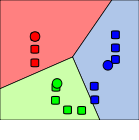
\includegraphics[width=\textwidth]{Images/Methods/K-means/K_Means_Example_Step_4.png}
        \vspace{-15pt}
        \caption{With the new centroids, the assignment step is again taken.}
    \end{subfigure}
    \caption{K-means clustering representation. This process is repeated until every centroid remains constant. Images from $Wikipedia$: $https://en.wikipedia.org/wiki/K$-$means\_clustering$. \\}
\end{figure}
The selection of the number of clusters is usually done by hand, but a good method to find out which k fits the model best is the $elbow$ $method$. 
The loss function is calculated for a varying number of clusters, and by plotting the result for each number of clusters, the goal is to look at the graph and find a vertex (the elbow). The $elbow$ represents a point at which further clustering does not significantly improve performance because the cost function decreases more slowly. In the next example (Figure 2.4), k-means was applied for different k values.
\begin{figure}[h!]
    \centering
    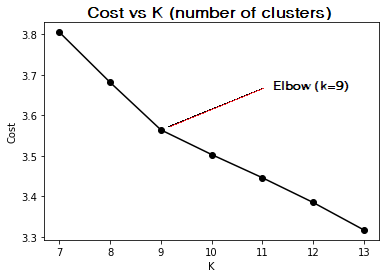
\includegraphics[scale=0.7]{Images/Methods/K-means/Fingerprints_elbow.png}
    \caption{Plotted cost function as a function of k. A clear elbow is found at k=9.}
\end{figure}


\subsubsection{Hierarchical Clustering}
On the other hand, hierarchical clustering is another approach that does not require the number of clusters to be fixed. Moreover, it is a very visual algorithm that provides a dendrogram, a "tree diagram showing taxonomic relationships". Here we explain the most common type of hierarchical clustering, agglomerative clustering. In this case, the dendrogram is built from the bottom up, starting with the single leafs up to the trunk \cite{James2013}.\\
 
Agglomerative clustering algorithms start with each observation forming a single cluster. N-1  times (in the case of N observations), the closest (most similar) pair of clusters is merged into a single cluster so that there is one less cluster at the next higher level. For this purpose, a distance measure between two clusters must be defined to set the criteria for merging them \cite{hastie01statisticallearning}. 

\begin{figure}[h]
    \centering
    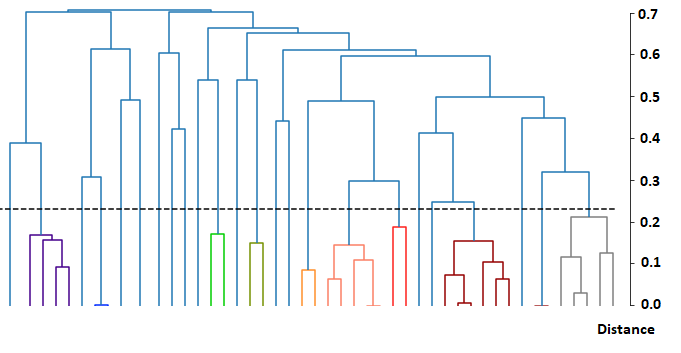
\includegraphics[scale=0.8]{Images/Methods/Hierarchical/Hierarchical dendogram.png}
    \caption{Example dendrogram with cluster criterion set. Each colour represents a cluster.}
\end{figure}


In hierarchical clustering, there are different types of linkage that take into account the distance between clusters. Imagine we have two clusters, A and B. The distance or dissimilarity measure is determined by considering the observations in each cluster in different ways:

\begin{itemize}
    \item \textbf{Ward linkage}: The objective of the Ward linkage criterion is to minimise within cluster variance. Therefore, in Ward linkage hierarchical clustering, the distance between clusters is determined based on the amount of variance increase that the merging of adjacent clusters A and B would lead to \cite{ward}.
    \item \textbf{Single linkage}: In single linkage hierarchical clustering, the distance between clusters is determined by the minimum distance between points of neighbouring clusters A and B.
    $$
    \min \{ d(a, b): a \in A, b \in B \}.
    $$
    \item \textbf{Complete linkage}: In complete linkage hierarchical clustering, the distance between clusters is determined by the maximum distance between points of adjacent clusters A and B.
    $$
    \max \{ d(a, b): a \in A, b \in B \}.
    $$
    \item \textbf{Average linkage}: In average linkage hierarchical clustering, the distance between clusters is determined by the average distance between all points of adjacent clusters A and B. $|A|$ and $|B|$ correspond to the number of observations in each cluster.
    $$
    \frac {1}{|A|.|B|}\sum_{a \in A}\sum_{b \in B}d(a, b).
    $$
    \item \textbf{Centroid linkage}: In centroid linkage hierarchical clustering, the distance between clusters is determined by the distance between centroids of adjacent clusters A and B:
    $$|
    |c_{A} - c_{B}||,
    $$
    where $c_{A}$ and $c_{B}$ are the positions of centroids of clusters A and B, respectively.
\end{itemize}\hspace{15cm}\cite{hastie01statisticallearning}

\subsection{Feature Selection Algorithms}
The predictive performance of a model depends on the adequate management of features. When avoiding unnecessarily high correlations among features that are able to trigger multicollinearity\footnote{Multicollinearity is a phenomenon which occurs when one descriptor is linearly related to combinations of other descriptors in the dataset, and it can be therefore predicted.}, it comes to mind which features ought to be selected. In a problem with way too many variables, an efficient algorithm can come in handy when performing the reduction.
\subsubsection{Sequential Feature Selection}
One of the simplest feature selection algorithms is the sequential feature selection algorithm. This is a greedy algorithm, meaning that, at every step, it makes the locally optimal choice, without considering whether this locally optimal choice will generate the globally optimal result.

Given a model, as well as some metric $J$ we can use to evaluate the performance every feature for that model, such as its F score (Section 2.4.3) or the cross-validation score of the model, the sequential feature selection algorithm chooses the $k$ best features for that model by following the procedure outlined below.

\begin{algorithm}[H]
\caption{Forward Sequential Feature Selection}
\begin{algorithmic}[1]
    \Require Set of all features $A=\{a_1, \dots, a_N\}$;
    
    Evaluation metric $J$;
    
    Target size of feature subset $M$.
    \Ensure Subset of best performing features $Y=\{y_1, \dots, y_M \}$.
    \State Start with empty set: $Y=\{\emptyset\}$.
    \For{$k \gets 1$ to $M$}
        \State Select next best feature: \[y_k = \argmax_{a_i\notin Y}{J(Y\cup a_i)}\]
        \State Add that feature to the feature subset: $Y=Y\cup y_k$.
    \EndFor
\end{algorithmic}
\end{algorithm}

That is, at every step, the algorithm evaluates the performance of every feature, then adds the best performing one to the final feature subset. It then repeats this procedure with all remaining features, until the predefined number of features is reached.\\

This algorithm can also be run backwards, where instead of starting from an empty set, $Y=\{\emptyset\}$, we instead start with a set that contains all features, $Y=X$. Then, at every step, rather than adding a new feature to the set, we instead remove the worse performing feature from it.\\

Sequential feature selection has certain advantages, such as its simplicity and speed, which makes it quite useful in scenarios where performance is a concern. However, it does have the disadvantages that it does not necessarily find the best possible subset of features for our model, and that a predefined number of features has to be chosen.


\section{PCA and Standardisation}
Also, whenever a large set of correlated variables has to be handled, principal components serve to summarise this group with a smaller number of representative variables that reflect all the variance of the original set of data on the whole. Principal components analysis (PCA) focuses on the method of calculating the principal components and the subsequent use of these components to understand the data. In addition to this, PCA also serves as a data visualisation tool, reducing the dimensionality of the data. It can also be used as a tool for data mapping, i.e. to fill in missing values in a data matrix. The issue is that each of the n observations occupies a p-dimensional space, but not all of these dimensions are of equal interest. PCA aims to find a small number of as interesting dimensions as possible, where the sense of interesting is determined by the degree of variance of the observations across each given dimension. Each of the dimensions found by PCA is a linear composition of the p features.\\

To perform PCA, variables must be centred and have a mean of zero. In addition, the results of PCA also depend on whether the variables have been scaled individually (each multiplied by a different constant). Since it is not advisable for the derived principal components to be based on an arbitrary choice of scaling, each variable is usually scaled so that it has a standard deviation of one before PCA is performed \cite{James2013}. 




\section{Evaluation Metrics}
Once the features are conditioned and established, it is time to properly evaluate each model and the content that corresponds to it, either to proceed with training or to evaluate the final version of the model itself.\\

For this, regression and correlation metrics are defined, as well as the feature evaluation metrics. 

\subsection{Regression Metrics}
Regression metrics are those that evaluate the performance of the algorithm, and are sometimes used by the algorithm itself to find the best possible version that is subsequently output.
Different regression metrics and algorithms that implement it are trying to solve different problems with distinct objectives. Each of these regression metrics are to be used most efficiently in the indicated cases, so the context needs to be taken into account. 
\subsubsection{Mean Absolute Error}
The mean absolute error (MAE) is defined by the sum of subtracting all the ``regressionwise" obtained values $\hat{y}_i$ from the real values $y_i$, and dividing the result by the number of observations $N$. Sometimes, a small change in an experiment can alter the result in a huge way, giving very wrong observations. While the rest of the data is still useful, estimations can be thrown off because of these observations. This regression metric is known for being keen with outliers (compared to the ones discussed later on), this means, it is apt to use in a datasets with possible mistakes and where the data may wrongly deviate. MAE is defined by the following formula:
\begin{equation}
  MAE=\frac{1}{N}\sum_{i=1}^N|y_i-\hat{y}_i|.  
\end{equation}
\subsubsection{Root Mean Squared Error}
When talking about root mean squared error (RMSE) mean squared error needs to be understood first. Mean squared error (MSE) is the simplest metric, and also the most used, even though its interpretation can be the most useless, as it depends on the scale of the problem and it can not be of good use when comparing with other models quantitatively. It is defined by the equation:
\begin{equation}
MSE=\frac{1}{N}\sum_{i=1}^N(y_i-\hat{y}_i)^2,
\end{equation}
where $y_i$ is the actual value and $\hat{y}_i$ is the predicted.
This metric is a very sensible metric to outliers in the data, therefore, the data should be trustworthy for implementing it, not like in MAE. RMSE is just the square root of MSE:

\begin{equation}
RMSE=\sqrt{\frac{1}{N}\sum_{i=1}^N(y_i-\hat{y}_i)^2}.
\end{equation}

As we can observe, 
$$
MSE(a)>MSE(b)\Longleftrightarrow RMSE(a)>RMSE(b).
$$

\subsubsection{Mean Absolute Percentage Error}
The mean absolute percentage error (MAPE) provides an understanding of the mean absolute error in a scaled representation, which can be easier to interpret when comparing among errors in data with different scaling.

Here is the formula for MAPE:
\begin{equation}
MAPE=\frac{1}{N}\sum_{i=1}^N\left|\frac{y_i-\hat{y_i}}{y_i}\right|.
\end{equation}

\subsection{Correlation Metrics}
The association between two variables, the way they mutually connect with each other is called correlation. The ways to measure this correlation are numerous, and while some explore the cardinal nature, some other also explore the ordinal nature of the values.\\

Four correlation metrics are going to be explained: Pearson, limiting coefficient ($R^2$), Spearman and Kendall rank coefficient. 

\subsubsection{Pearson Correlation}

The simplest way to look at whether two variables are associated is to look at whether they ``covary". If we are interested in whether two variables are related, then we are interested in whether changes in one variable are met with similar changes  in  the  other  variable.  Therefore,  when  one  variable  deviates  from  its  mean  we would expect the other variable to deviate from its mean in a similar way. The measurement of the similarity in the pattern of two random variables is closely related to the concept of variance. Variance measures how far a set of numbers is spread out from their average value (deviance), and is calculated as follows:

\begin{equation}
Var(X) = \frac{\sum(x-\bar x)^{2}}{N-1},
\end{equation}
where the square of the deviance is taken to avoid negative and positive deviances canceling each other out.

If we want to understand how two variables covary, we can multiply the deviance of both variables.

\begin{equation}
Cov(X, Y) = \frac{\sum(x-\bar x)(y-\bar y)}{N-1}.
\end{equation}

A  positive  covariance  indicates  that  as  one  variable  deviates  from  the  mean, the other variable deviates in the same direction. On the other hand, a negative covariance indicates that as one variable deviates from the mean, the other deviates from the mean in the opposite direction.

An important thing to note is while covariance tells us what the "direction" of the relationship between two variables is (whether they increase/decrease in the same or opposite directions), it doesn't tell us about the "strength" of the relationship (how closely related these increases/decreases are). This is because covariance isn't a standardised measurement. We can see an example of this phenomenon below.

A common way to address the problem with covariance we just described is to standardise the covariance by dividing by the standard deviations.

\begin{equation}
\rho_{p}(X, Y) = \frac{\sum(x-\bar x)(y-\bar y)}{(N-1)\sigma_{x}\sigma_{y}}=\frac{Cov(X,Y)}{\sigma_{x}\sigma_{y}}.
\end{equation}

This coefficient is called Pearson's correlation, and it takes values between -1 and 1. Below we can see that the phenomenon observed with covariance is not a problem with correlation.

\subsubsection{Limiting coefficient}

One disadvantage of the Pearson's correlation metric is that it is difficult to compare different correlation values with each other. For instance, it is not obvious that a model with 0.9 correlation is twice as good at making predictions as a model with 0.64 correlation.

Another common metric to measure correlation is the coefficient of determination or $R^{2}$. This metric has a few advantages over Pearson's correlation, namely that it's values can be directly compared, and that it can be interpreted as the percentage of the total variance of the response variable that is explained by our model.

To understand how to calculate this metric, we will first look at a few definitions.
\begin{wrapfigure}{r}{0.5\textwidth}
\begin{center}
\vspace{-1cm}
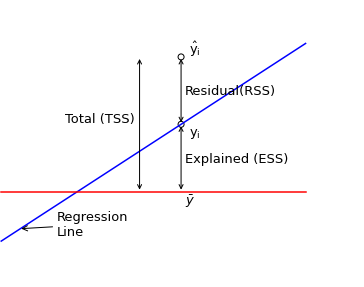
\includegraphics[scale=0.75]{Images/Methods/Correlation/R2_Plot.png}
\caption{\centering Graphic representation of TSS, RSS and ESS.}

\vspace{-1cm}
\end{center}
\end{wrapfigure}
\begin{itemize}
  \item $TSS$ or Total sum of squares: the average squared error between the true value $y_{i}$ and the average $\bar y$.
  \item $RSS$ or Residual sum of squares: the average squared error between the true value $y_{i}$ and the predicted value $\hat y_{i}$ (Equation \ref{eqn:RSS}).
  \item $ESS$ or Explained sum of squares: the average squared error between the predicted value $\hat y_{i}$ and the $\bar y$.
\end{itemize}


The most general definition of the coefficient of determination is given by:

\begin{equation}
R^{2} = 1 - \frac{RSS}{TSS} = \frac{ESS}{TSS}.
\end{equation}

In other words, $R^{2}$ being high means that a high percentage of the total variance is the response variable is explained by the model. A baseline model that always predicts $\bar y$ will have a $R^{2}=0$. $R^{2}$ can have values below zero if the predictions are below this baseline.

It must be kept in mind that these measures of correlation only account for linear dependencies between variables, that is, relationships of the form:

\begin{equation}
    Y = \beta_{0}X_{0} + \beta_{1}X_{1} + \dots + \beta_{k}X_{k}.
\end{equation}

We can observe this phenomenon in the following examples of Figure 2.7.

\begin{figure}[h!]
\centering
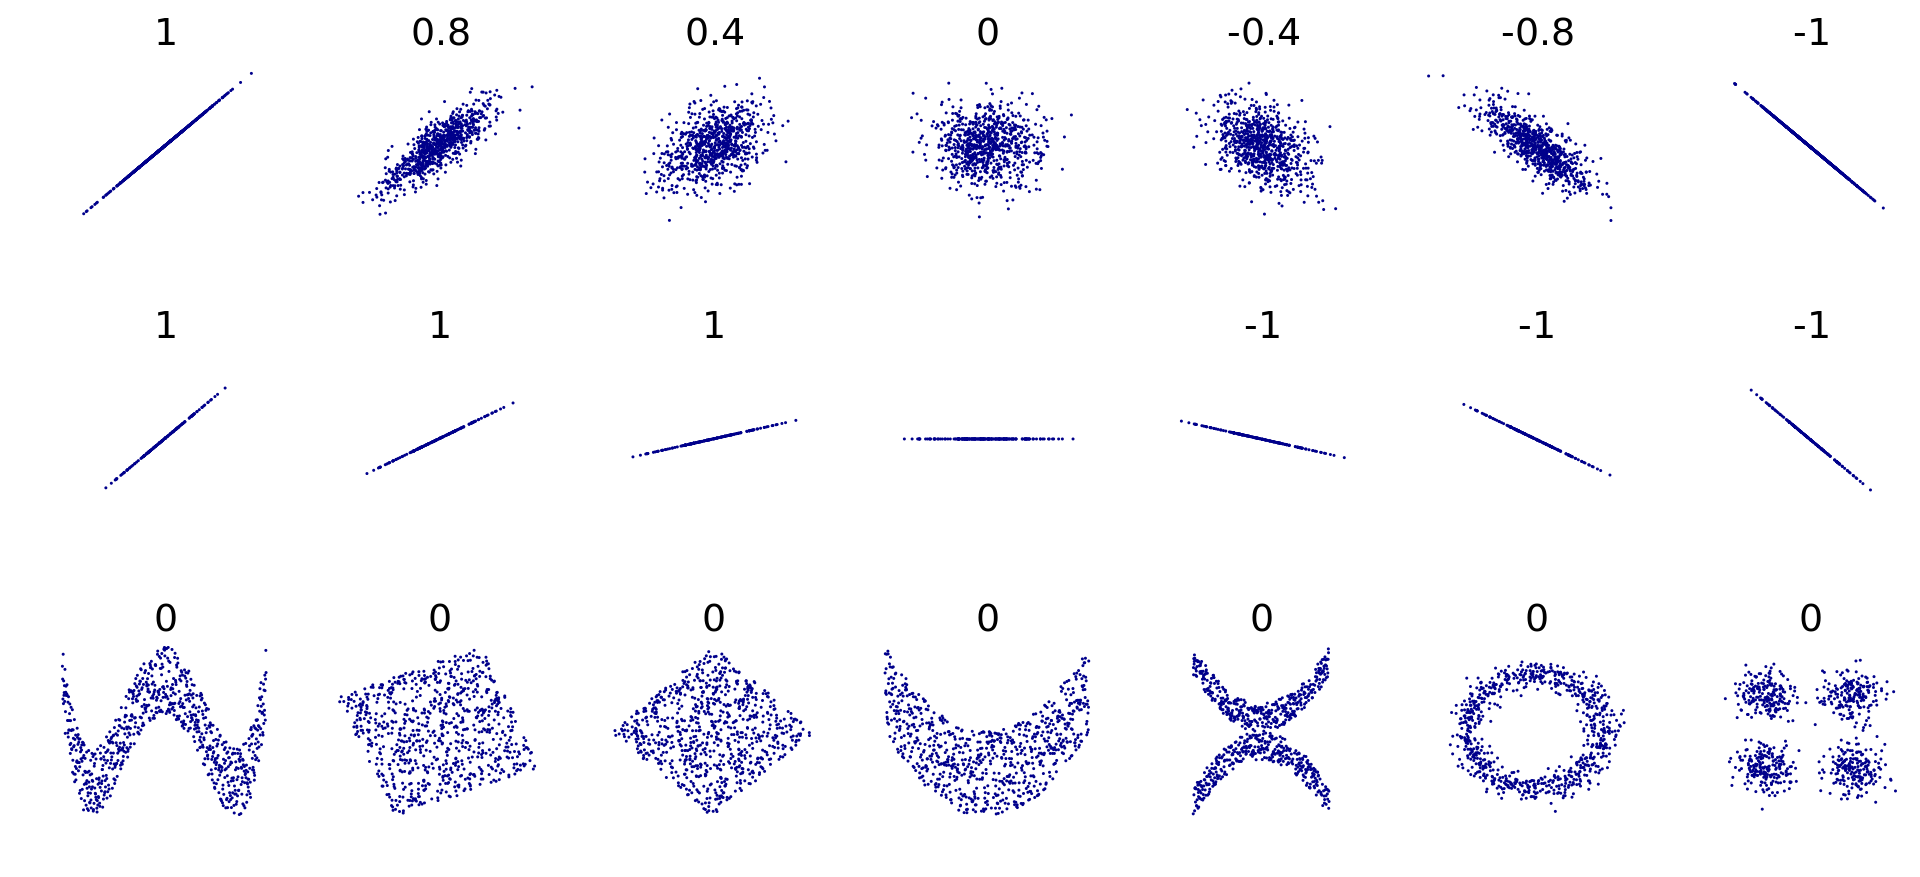
\includegraphics[scale=0.2]{Images/Methods/Correlation/CorrelationValues.png}
\caption{Examples of different R² values.}
\end{figure}    


\subsubsection{Spearman Correlation}
The correlation measures explained above take into account linear dependencies, but do not describe non-linear ones. For this, Spearman's Correlation is defined, which explores the dependencies of the ordinal nature of the given data, rather than the data measure itself. For this, ranks are established, where instead of calculating the correlation of the original variables, the correlation of the ranks of the variables is calculated (Spearman, 1904).  Under the null hypothesis, each rank of X should have the same probability of being associated with each rank of Y. So in Spearman's correlation, it is the covariance between ranks that is taken into account, rather than the covariance between variables. Moreover, as in Pearson's correlation, they are always divided by the respective standard deviations of the ranks:

\begin{equation}
    \rho_s(X,Y)=\frac{\sum(R(x)-N/2)(R(y)-N/2)}{(N-1)\sigma_{R(x)}\sigma_{R(y)}}=\frac{Cov(R(X),R(Y))}{\sigma_{R(X)}\sigma_{R(Y)}}.
\end{equation}

Otherwise, Spearman's correlation is Pearson's correlation in ranks.

Pearson (1907) criticises the Spearman correlation on the grounds, among others, that since it is designed to reflect the relationship even if the relationship is not linear, it also loses the possibility of being considered a regression parameter even if the underlying relationship is linear \cite{Kolassa2020}.

\subsubsection{Kendall Rank Correlation Coefficient}
Another correlation metric that takes into account the ordinal nature of the data is the Kendall rank correlation coefficient, also known as Kendall's $\tau$. To understand the underlying principle of this correlation metric, concordant and discordant pairs need to be defined. Bivariate observations for which the X and Y values are in the
same order are called concordant; pairs that are not concordant are called discordant.\\

Kendall's $\tau$ builds a new calculation which is based on the 
counts of concordant and discordant pairs. The concordant pair number U:
\begin{equation}
    U=\sum_{i<j}^NZ_{ij},
\end{equation}
where\\
\begin{equation}
    Z_{ij}=
    \begin{cases}
    1,\hspace{1.2cm} (X_j-X_i)\cdot(Y_j-Y_i)>0\\ 
    0,\hspace{1.2cm} (X_j-X_i)\cdot(Y_j-Y_i)<0
    \end{cases}.
\end{equation}

Therefore, Kendall's $\tau$ is evaluated subtracting the number of discordant pairs from U, the number of concordant pairs, and then dividing this by the number of ways to choose two items from n items, ${n \choose 2}=n(n-1)/2$ :
\begin{equation}
    \tau= \frac{U-\left({n\choose2}-U\right)}{{n\choose2}}=\frac{4U}{n(n-1)}-1.
\end{equation}\hspace{15cm}\cite{Kolassa2020}
\subsection{Feature Evaluation Metric}
Evaluation of the features themselves is an important part of the machine learning problems.  
In Section 2.2.4, the sequential feature selection algorithm was explained, as well as the reason for its implementation. These models which were worked on implement the feature evaluation metric explained below: F Score.
\subsubsection{F Score}
F Score is a useful and simple evaluation metric specially used for features, where the Pearson correlation between the response and descriptor features is calculated one by one.\\

The descriptors with highest correlation with the response feature are determined to be the ones that have valuable information referring to the response feature, and they therefore have higher scores. 


\section{Model Evaluation}
The process of evaluating whether the model is good or bad enough can be harsh. Feedback in the data used for training the algorithm, such as RSS (or other metrics) that was minimised, does not always provide a full sight of the righteousness of the model; data which is influential in the building of the model does not supply a valuable enough response on whether it will work on raw, virgin data. Therefore, to be able to evaluate afterwards, the data itself has to be separated in a \textbf{training set}, which is used to feed the algorithm; and \textbf{test set}, which is used one and only for the appraisal of the model built. 
\subsection{Learning Curves}
Using learning curves, plenty can be learnt from a model. Inspecting the shape of these can show whether a model is overfit or underfit, depending on the variable chosen. Two curves are set, the test error curve and the training error curve. The test error is the average error that results from using the test set. It is obvious that given a dataset, the use of a particular statistical learning method is warranted if it results in a low test error. The training error is the error obtained in the training set. A low training error with a high test error is a clear result of overfitting (Figure 2.6), while the opposite, a relatively high training error with a lower test error is subject to underfitting (Figure 2.7).
\begin{figure}[h!]
  \centering
  \begin{minipage}[b]{0.45\textwidth}
    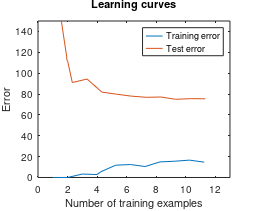
\includegraphics[width=\textwidth]{Images/Methods/Evaluation/overlc.png}
    \caption{Overfitting model.}
  \end{minipage}
  \hfill
  \begin{minipage}[b]{0.45\textwidth}
    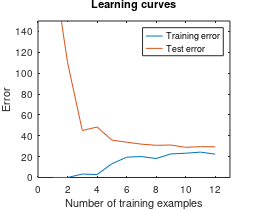
\includegraphics[width=\textwidth]{Images/Methods/Evaluation/goodlc.png}
    \caption{Underfitting model.}
  \end{minipage}
\end{figure}\\

Learning curves can be used for hyperparameter tuning because the optimal hyperparameter value can be chosen to fit neither too well nor too poorly, with as little training and testing error as possible. They can also be plotted as a function of the size of the training set, as in Figures 2.8 and 2.9. These types of learning curves can also show whether the current model is underfitting or overfitting, as well as the potential performance of the model when trained with a larger dataset, since the evolution of these curves as more training examples are added can be predicted by simple observation.

\subsection{Cross-Validation}
The test error can be easily calculated if a specific 
test set is available. Unfortunately, this is usually not the case. In contrast, the training error can be easily calculated by applying the statistical learning method to the observations used in training. The training error rate is often significantly different from the test error rate, and in particular the training error rate can drastically underestimate the test error rate.
\subsubsection{K-Fold Cross-Validation}
K times repeated k-fold cross-validation is commonly used to evaluate the predicted
performance on different predicted models \cite{YUAN2022100026}. In this form of cross-validation, switching portions of data are used to train and to test the models k times.\\

 Figure 2.10 shows a more visual representation of the process. 
\begin{figure}[h!]
    \centering
    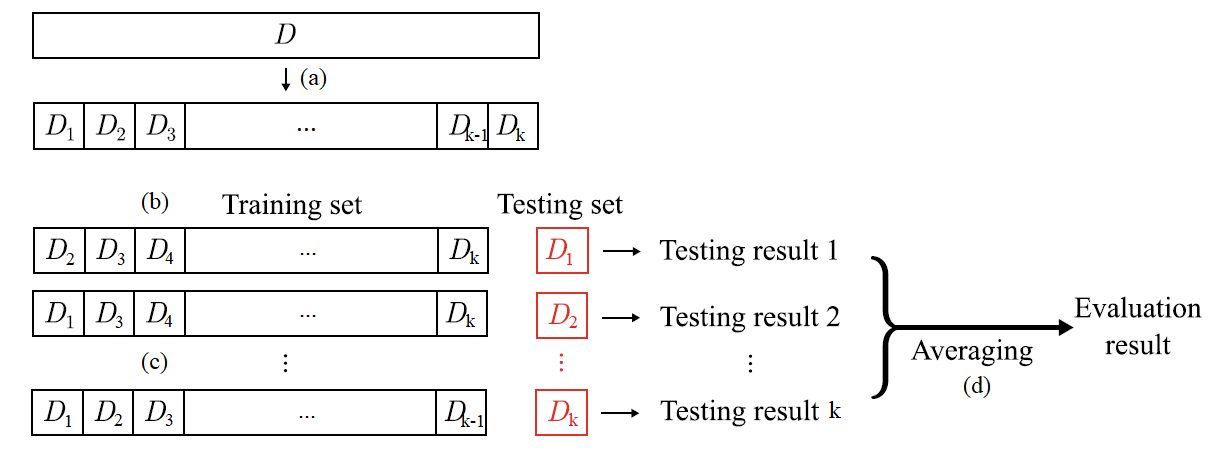
\includegraphics[width=0.7\textwidth]{Images/Methods/CV/Kfcv.png}
    \caption{K-fold cross-validation process. The dataset is broken down in k different subsets, with roughly the same size (a). K-1 subsets are used as training sets, for the algorithm to train itself on, while the remaining subset is used for test (b). The error obtained in this test subset is noted. This process is carried on k times, using each subset as test only once (c), and the mean value of the error is obtained by averaging (d), providing a more precise estimation for the error \cite{Zhou21a}.}
\end{figure}

\subsection{Bootstrapping}
When having used a dataset of size D, the previous method does not offer a chance to evaluate a method trained on D observations, simply because part of these D observations are spared in order to serve as testing virgin data. This provokes an unavoidable estimation bias, specially in the case of smaller datasets, where sparing one observation alone can be able to overthrow the estimation. For these cases, $bootstrapping$ is a solution.\\

In bootstrapping, a new dataset is created, and D observations from the original dataset are randomly put in the new dataset. Sampling without replacement is the way to go, as the same observation can be repeatedly be copied. In this way, we can create a new bunch of same size and different datasets which can be very useful to train and evaluate the model (not reducing the training set size).

\subsubsection{Confidence interval}
Another thing that can be done when wanting to calculate the mean value of the observations, is plotting a histogram of the mean values obtained in each dataset. The more the new datasets, the better the understanding of the actual mean value and its error. This way, we can create intervals in the histogram that encompass a different amount of confidence, and are subsequently called confidence intervals. An 80\% confidence interval, for example, would include 80\% of the mean values calculated through the different datasets (original and new). 

\subsection{Nested Cross-Validation}
A more efficient but computationally expensive evaluation method is nested cross-validation, where a combination of k-fold cross-validations and bootstrapping allows for a more accurate and reliable estimation of the performance. This is why this was the performance guideline evaluation method used in this problem.\\

In nested cross-validation (see Figure 2.11) , 10-fold cross-validation is carried on where training and test sets are generated from the data, this is called the $outer$ $loop$. This training sets are then separated into training and validation sets using 5-fold cross-validation on which is determined to be the $inner$ $loop$. The training sets are used to train the model, utilising the feature selection algorithm, and grid search is used to determine which hyperparameter values fit the model with least error, for these last two, the validation set mentioned beforehand is used.\\\\ 
--------------------------------------------------------------------------------------------------------------------
\subsubsection{Grid Search}
Grid search is used to find the optimal hyperparameter value in the model for the selected dataset. The model is trained with the training set for different hyperparameter values, and the error is calculated for the validation set in each combination.\\

For this, after the learning curve is plotted, it usually happens that it is not clear which value to set as the optimal one. The goal of grid search is to search among a value stretch to choose the one which minimises the error in the validation set. The stretch selected is divided in the selected number $n$, and the different $n$ values are tested.\\

For example, imagine it is not clear which values for number of trees from 0 to 100 and maximum depth of the trees from 2 to 5 best fit the dataset in Random Forest regression.
$n_1$=21 and $n_2$=4 can be chosen, and the values tested would be: 0,5,10,15,20,...,95,100, for number of trees; and 2,3,4,5, for the maximum depth of these trees.
94 (21x4) individual combinations can be tested, the validation set is meant to select the optimal one in the metric chosen.\\\\
\begin{wrapfigure}{r}{0.6\textwidth}
\begin{center}
\vspace{-1.7cm}
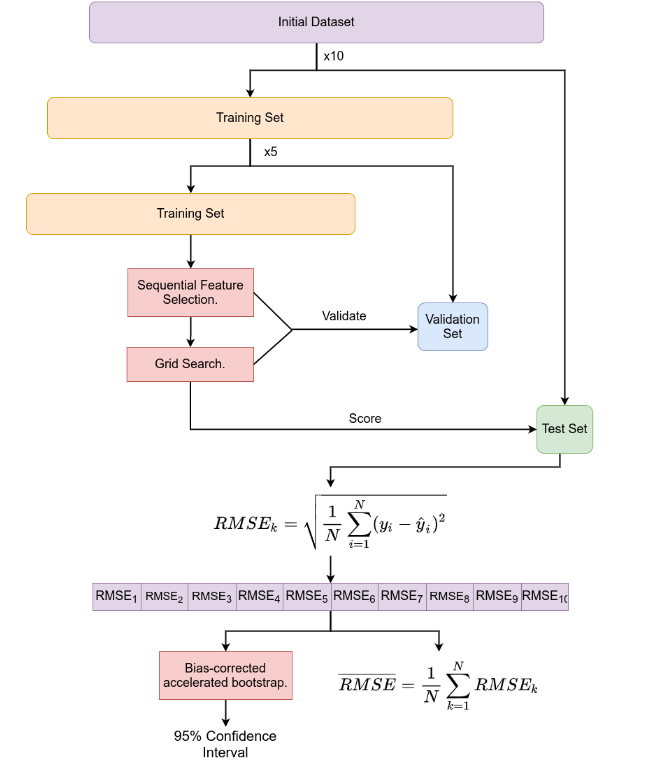
\includegraphics[width=0.6\textwidth]{Images/Methods/CV/Nested CV.png}
\caption{\centering Nested cross-validation diagram.}
\vspace{-1cm}
\end{center}
\end{wrapfigure}
---------------------------------------------\\


The outer test set is used now for the first time. A virgin dataset is needed (validation set was used in grid search and feature selection) to calculate the metric wanted to be determined (RMSE in Figure 2.11) without the influence on which the model was optimised.\\

 With the 10 values obtained (for each fold), on the one hand, a mean value is calculated; on the other hand, bootstrapping is applied to get a 95\% confidence interval. Also, the minimum and maximum values among the 10 values are noted.

\subsection{Reliability}
The reliability of the model is very important after having optimised the algorithm. Comparing hypotheses or models is what is usually done to get a frame of reference of the quality and reliability of the algorithm.   
\subsubsection{Paired Sample T-Test} 
When dealing with two models' results and wanting to compare them, the paired sample t-test provides a viewpoint for when we are concerned about the difference between two variables surrounding the same subject.
This is the formula for the t statistic:
\begin{equation}
    t=\frac{\overline{x_1}-\overline{x_2}}{\sqrt{\frac{\sigma_1}{n_1}+\frac{\sigma_2}{n_2}}},
\end{equation}
where $\overline{x}$ is the mean value for the variable, $\sigma$ is the standard deviation and n accounts for the data points. The suffixes 1 and 2 refer to each hypothesis tested.
\subsubsection{Empirical p-values}
P-values define the probability that a t statistic, or higher, would be obtained from the t distribution.\\

The percentage of error that we are willing to run our test with each one of the hypothesis is the significance $\alpha$. It can be set to whichever value wanted, but the most usual is 0.05, equivalent to 5\%, for hypothesis testing. Consequently, a p-value smaller than $\alpha$ discards the equivalence \cite{pvalue}. 
 

 














\chapter{Application}
\hspace{1.5cm}The application of machine learning techniques implies a personal and subjective role, namely the selection of the features that can best describe the context of the response variable. The context is not insignificant, it is the most important part of this process. The more valuable the information fed to the algorithm, the more accurate the construction of the model.\\\\
The data used to construct the models in this work was obtained through the site BindingDB.org, which is a database of measured binding affinities of protein considered to be drug-targets (receptors) with small, drug-like molecules (ligands). The database contains experimental information about the binding affinities of 175 inhibitors of the SK4 potassium channel, measured as half-maximal inhibitory concentration ($\text{IC}_{50}$(nM)).\\

\textbullet\hspace{0.1cm} \textbf{$\text{IC}_{50}$}: necessary concentration of the ligand that is necessary to achieve 50\% inhibition of the receptor.\\

The $\text{IC}_{50}$ was in fact the measure that we attempted to model in this work. More precisely, the logarithm of the $\text{IC}_{50}$ (p$\text{IC}_{50}$) was modeled, since we observed that the distribution of the $\text{IC}_{50}$ in our dataset was heavily skewed, which can cause problems when constructing models. Meanwhile, the p$\text{IC}_{50}$ has a much more convenient Gaussian-like distribution, as can be seen in Figure 3.1.\\

\begin{figure}[h]
    \centering
    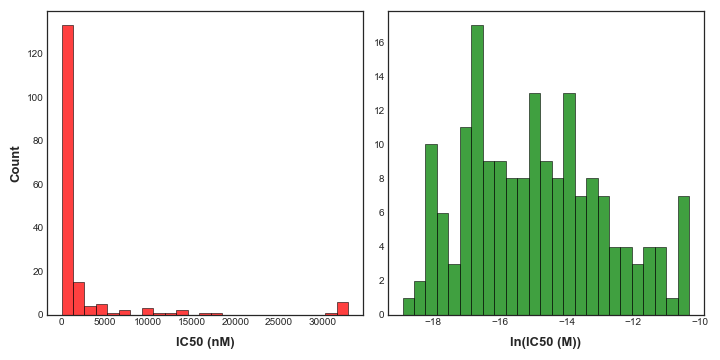
\includegraphics[width=14cm, height=5.7cm]{Images/Results/Feature Analysis/IC50_distributions.png}
    \caption{Histograms of the distributions of the $\text{IC}_{50}$ (left) and its logarithm (right) for the dataset of ligands used in this work.}
\end{figure}

\section{Feature Analysis}
The feature obtaining and management were, as stated, uppermost important parts of this process, as the outcome depends on how  most data is retained whilst being consequent on the significance of each feature. The way to do this guards itself on setting, in some way, how important we want each feature to be, based on the weighing of how relevant it is (positively) to the outcome itself. 

\subsection{Features}
In order to build the models we are interested in, the features extracted beforehand can be divided, broadly speaking, into two groups: features related to the chemical characteristics of the ligands\footnote{These were obtained by the group, the Schrödinger software package was used \cite{maestro}.}, \textbf{chemical features}, and features related to the way in which the bound ligands interact with the receptor protein. These last features can furthermore be divided into \textbf{energetic features} and \textbf{SASA features}.\\

While chemical features were relatively easy to obtain, energetic features such as Van der Waals interactions or hydrogen bonds relating the ligand to the receptor protein, or SASA ($Solvent$-$Accessible$ $Surface$ $Area$) features relating the surface of the receptor accessible to the ligand before and after the linkage, were extracted by the group\footnote{The group used GLIDE software (more information in \cite{glide}).}$^,$\footnote{The group is referred to as in \cite{group}.}. The group performed what is called molecular docking (see Figure 3.2) of the 175 ligands to get the values for these energetic and SASA features. 

\begin{center}
    \begin{figure}[h]
    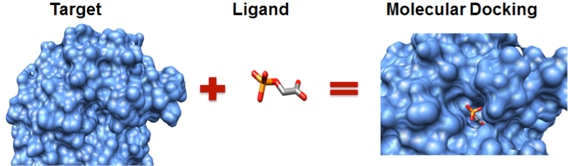
\includegraphics[width=15cm, height=4.5cm]{Images/Results/docking_image.jpg}
    \caption{Schematic illustration of the docking process for a ligand and its target. Image from \cite{docking_figure}.}
    \vspace{-10pt}
    \end{figure}
\end{center}
A total number of 48 descriptor features' data was extracted in the end. More information about some of the most relevant descriptors can be found in the appendix.

\subsection{Feature Conditioning}
Once the selected features' data was collected, PCA was performed on all data to observe how much variance was retained. For this, 17 principal components were obtained; the variance retained can be observed in Figure 3.3.\\\\   

\begin{figure}[h]
    \centering
    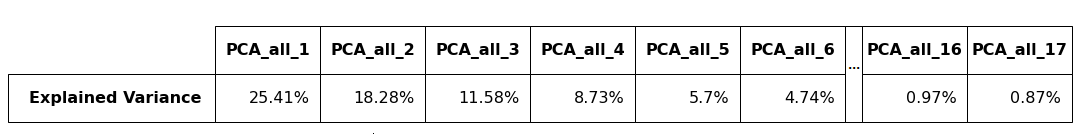
\includegraphics[width=\textwidth]{Images/Results/Feature Analysis/PCA_all variance.png}
    \caption{Observed variance in PCA of all features.}
\end{figure}
In these PCA, it can be assured 95.29\% of all variance was retained, while the first 8 principal components kept 81.6\%. The first 8 principal components were therefore saved, alongside the other 48 features.
As important as it may be holding on to the information on the data, it is also important that irrelevant or repeated data is not given the importance that it does not possess. 
Observing the Pearson correlation among features in Figure 3.4, it can be seen that many of these features are not just almost the same, but can be related to other features in many ways, as some rows (or columns) seem completely identical, and dark quadrants can be spotted in many places, respectively:
\begin{figure}[h]
    \centering
    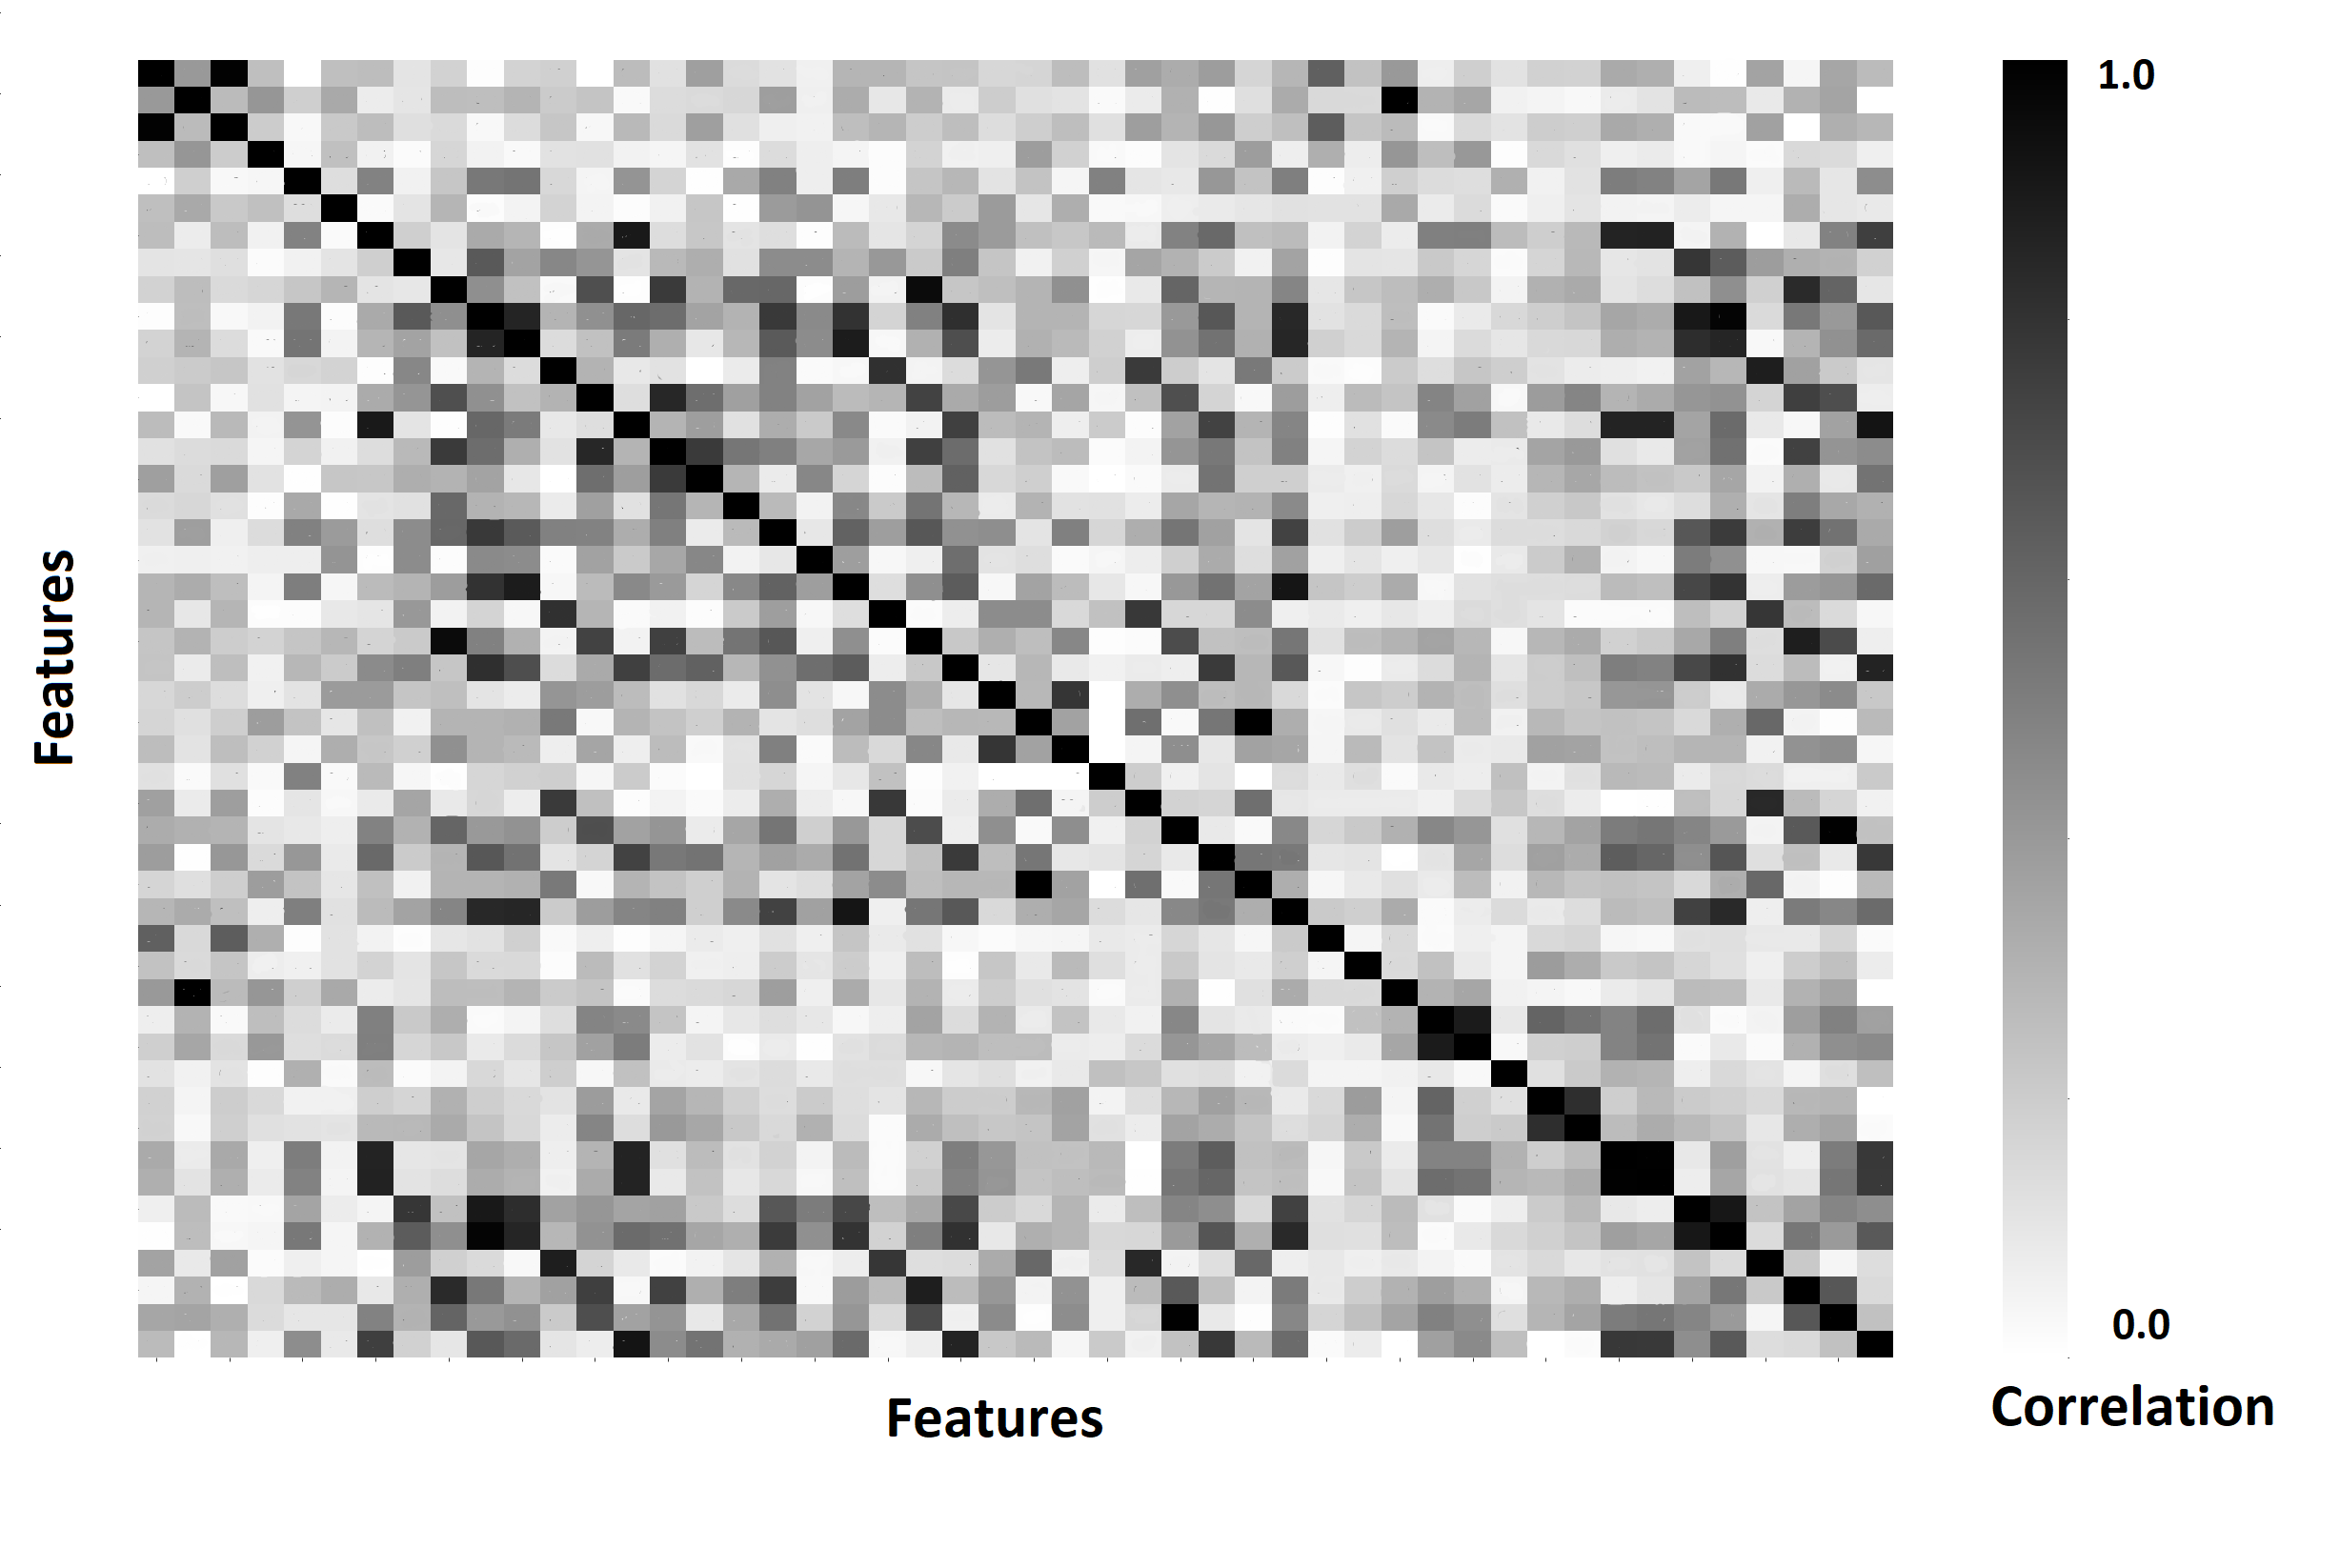
\includegraphics[width=0.6\textwidth]{Images/Results/Feature Analysis/feature correlation.png}
    \caption{Correlation amongst features.}
\end{figure}
\subsection{Feature Clustering}
To identify these correlations better, hierarchical clustering\footnote{It was decided the number of clusters ought to be chosen by a correlation threshold that gave better results, and not beforehand. K-fold clustering was given a try, but no elbow was clear.} was carried on all the features. All the different linkages were examined, as we can see in Table 3.1.
 \begin{table}[h!]
\resizebox{\textwidth}{!}{%
\begin{tabular}{ |p{3.5cm}||p{1.5cm}|p{2.8cm}|p{2.7cm}|p{2.7cm}|p{3.5cm}|  }
 \hline
&Number of\hspace{1cm} clusters &Mean\hspace{1cm} Within-Cluster Correlation&Mean\hspace{1cm} Out-of-Cluster Correlation&Standard\hspace{1cm} Out-of-Cluster Correlation&Number of Unclustered Correlations Above Threshold\\
 \hline
 Ward  linkage   & 13    &0.877856&   0.234071	&0.180442	&5\\
 Single linkage& 9& 0.664165	&0.200436	&0.151496	&0\\
 Complete linkage& 12 & 0.864345	&0.230020	&0.174760&3	\\
 Average linkage& 12 & 0.864345	&0.230020	&0.174760&3	\\
 Centroid linkage& 12  & 0.864345	&0.230020	&0.174760&3	\\
 \hline
\end{tabular}}
\caption{Models and correlations.}
\end{table}





After all the linkage types were explored, one was chosen as well as the appropriate threshold. In Table 3.1, where the obtained feedback for each linkage was obtained, it turns out that single linkage was the worst method (low internal correlation of clusters when creating a single giant cluster). The complete, average and centroid linkage methods obtained the same results, although they arrived at it by different routes. These results seemed slightly better than the Ward linkage, as there were less high correlations outside the cluster, but there was not a huge difference. 
The complete linkage method was chosen, and the dendrogram, as well as the matrix, plotted (Figure 3.5).\\
\begin{figure}[h!]
    \centering
    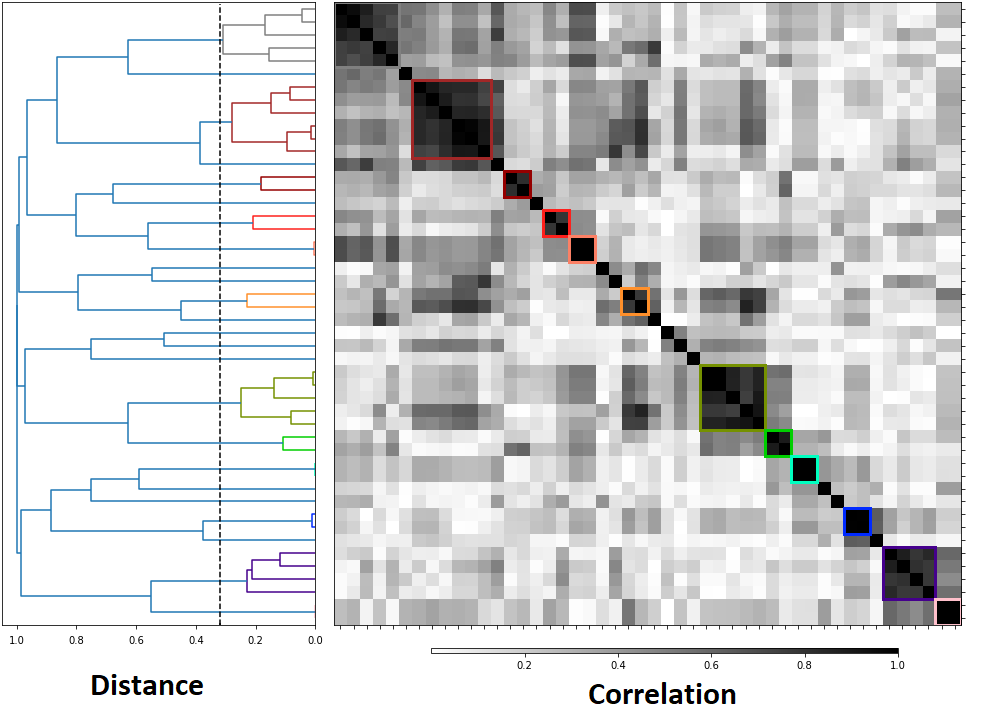
\includegraphics[width=0.8\textwidth]{Images/Results/Feature Analysis/h.complete.png}
    \caption{Complete linkage hierarchical clustering.}
\end{figure}

 Principal component analysis could then be performed on the features of each cluster. The goal was to obtain single features that represent a large percentage of the variance within each cluster. As in Section 3.1.2, the hope was that since a large percentage of the variance was retained, and most of the information of the features within the cluster was represented in these principal components. Clusters with three or more features were taken into account.\\
 \begin{figure}[h!]
    \centering
    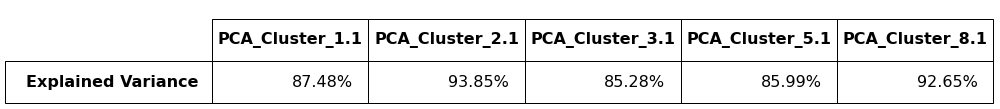
\includegraphics[width=\textwidth]{Images/Results/Feature Analysis/PCA cluster.png}
    \caption{Observed variance in cluster PCA.}
\end{figure} 


 To evaluate the situation with these new features, hierarchical clustering was then performed again. The threshold correlation within clusters was set to 0.68, by having done a grid search around the value, 0.68 was determined to be the most efficient threshold. \\\\
 
\begin{table}[h]
\resizebox{\textwidth}{!}{%
\begin{tabular}{ |p{3.5cm}||p{1.5cm}|p{2.8cm}|p{2.7cm}|p{2.7cm}|p{3.5cm}|  }
 \hline
&Number of\hspace{1cm} clusters &Mean\hspace{1cm} Within-Cluster Correlation&Mean\hspace{1cm} Out-of-Cluster Correlation&Standard\hspace{1cm} Out-of-Cluster Correlation&Number of Unclustered Correlations Above Threshold\\
 \hline
 Ward  linkage   & 13    &0.894085	&  0.228546		&0.187591		&8\\
 Single linkage& 6& 0.578955		&0.174990		&0.138137		&0\\
 Complete linkage& 12 & 0.884122		&0.226165		&0.184679	&8	\\
 Average linkage& 11 & 0.853568	&0.217090		&0.173517	&2	\\
 Centroid linkage& 11  & 0.853568	&0.217090		&0.173517	&2	\\
 \hline
\end{tabular}}
\caption{Models and correlations.}
\end{table}


This is the same as before, but this time the result was the same using the average and centroid linkage methods, and in both cases the number of points with high correlation was minimal as they form larger clusters. This time the centroid linkage method was chosen. The cluster matrix is shown in Figure 3.7. \\

\begin{figure}[h!]
    \centering
    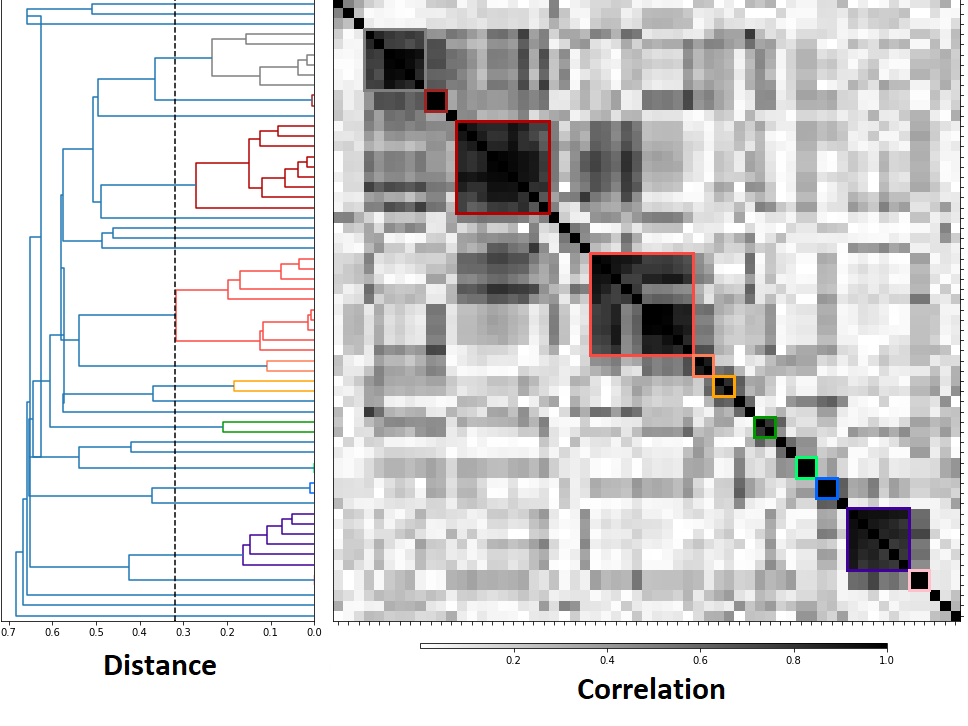
\includegraphics[width=0.8\textwidth]{Images/Results/Feature Analysis/centroid.png}
    \caption{Centroid linkage hierarchical clustering.}
\end{figure}




\subsection{Feature Selection}
These were too many features and a significant correlation could be found among them, so there was need to cut some off because they were only going to overestimate those correlated features.\\\\\\\\

\subsubsection{\hspace{8.85cm}F Score based selection}
\begin{wrapfigure}{l}{0.53\textwidth}
\vspace{-60pt}
\begin{center}
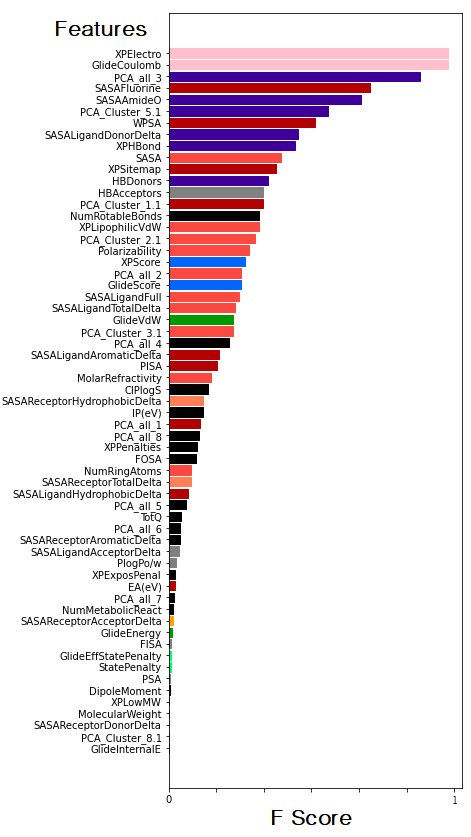
\includegraphics[width=0.50\textwidth]{Images/Results/Feature Analysis/fscore.png}
\caption{\centering Features' F score.}
\vspace{-20pt}
\end{center}
\end{wrapfigure}
For that, the F Scores were calculated for each feature as guides to help choose the best ones from each cluster. In Figure 3.8, the features' F score is observed, where the colour of each bar represents their corresponding cluster.\\

First, one of the of features in each cluster containing only two features was  eliminated. Some features have correlations close to 1, which means they are essentially the same features, so one can just be removed. For pairs of features with lower correlation, the decision was made based on which one has the highest F Score. These scores were calculated over and over again with each removal.
\subsubsection{Cluster correlation based selection}
Second, unnecessary features were eliminated within each cluster. The  correlation matrix of each cluster was plotted, with the goal of keeping as much information within the cluster while removing as many correlations as possible. Decisions were taken based on the F scores as well as the within-cluster correlations.\\

Having removed most of the correlations within the feature set, the correlation matrix (Figure 3.10) was redrawn, and compared to the one with all the features (Figure 3.9).
\begin{figure}[h!]
  \centering
  \begin{minipage}[b]{0.48\textwidth}
    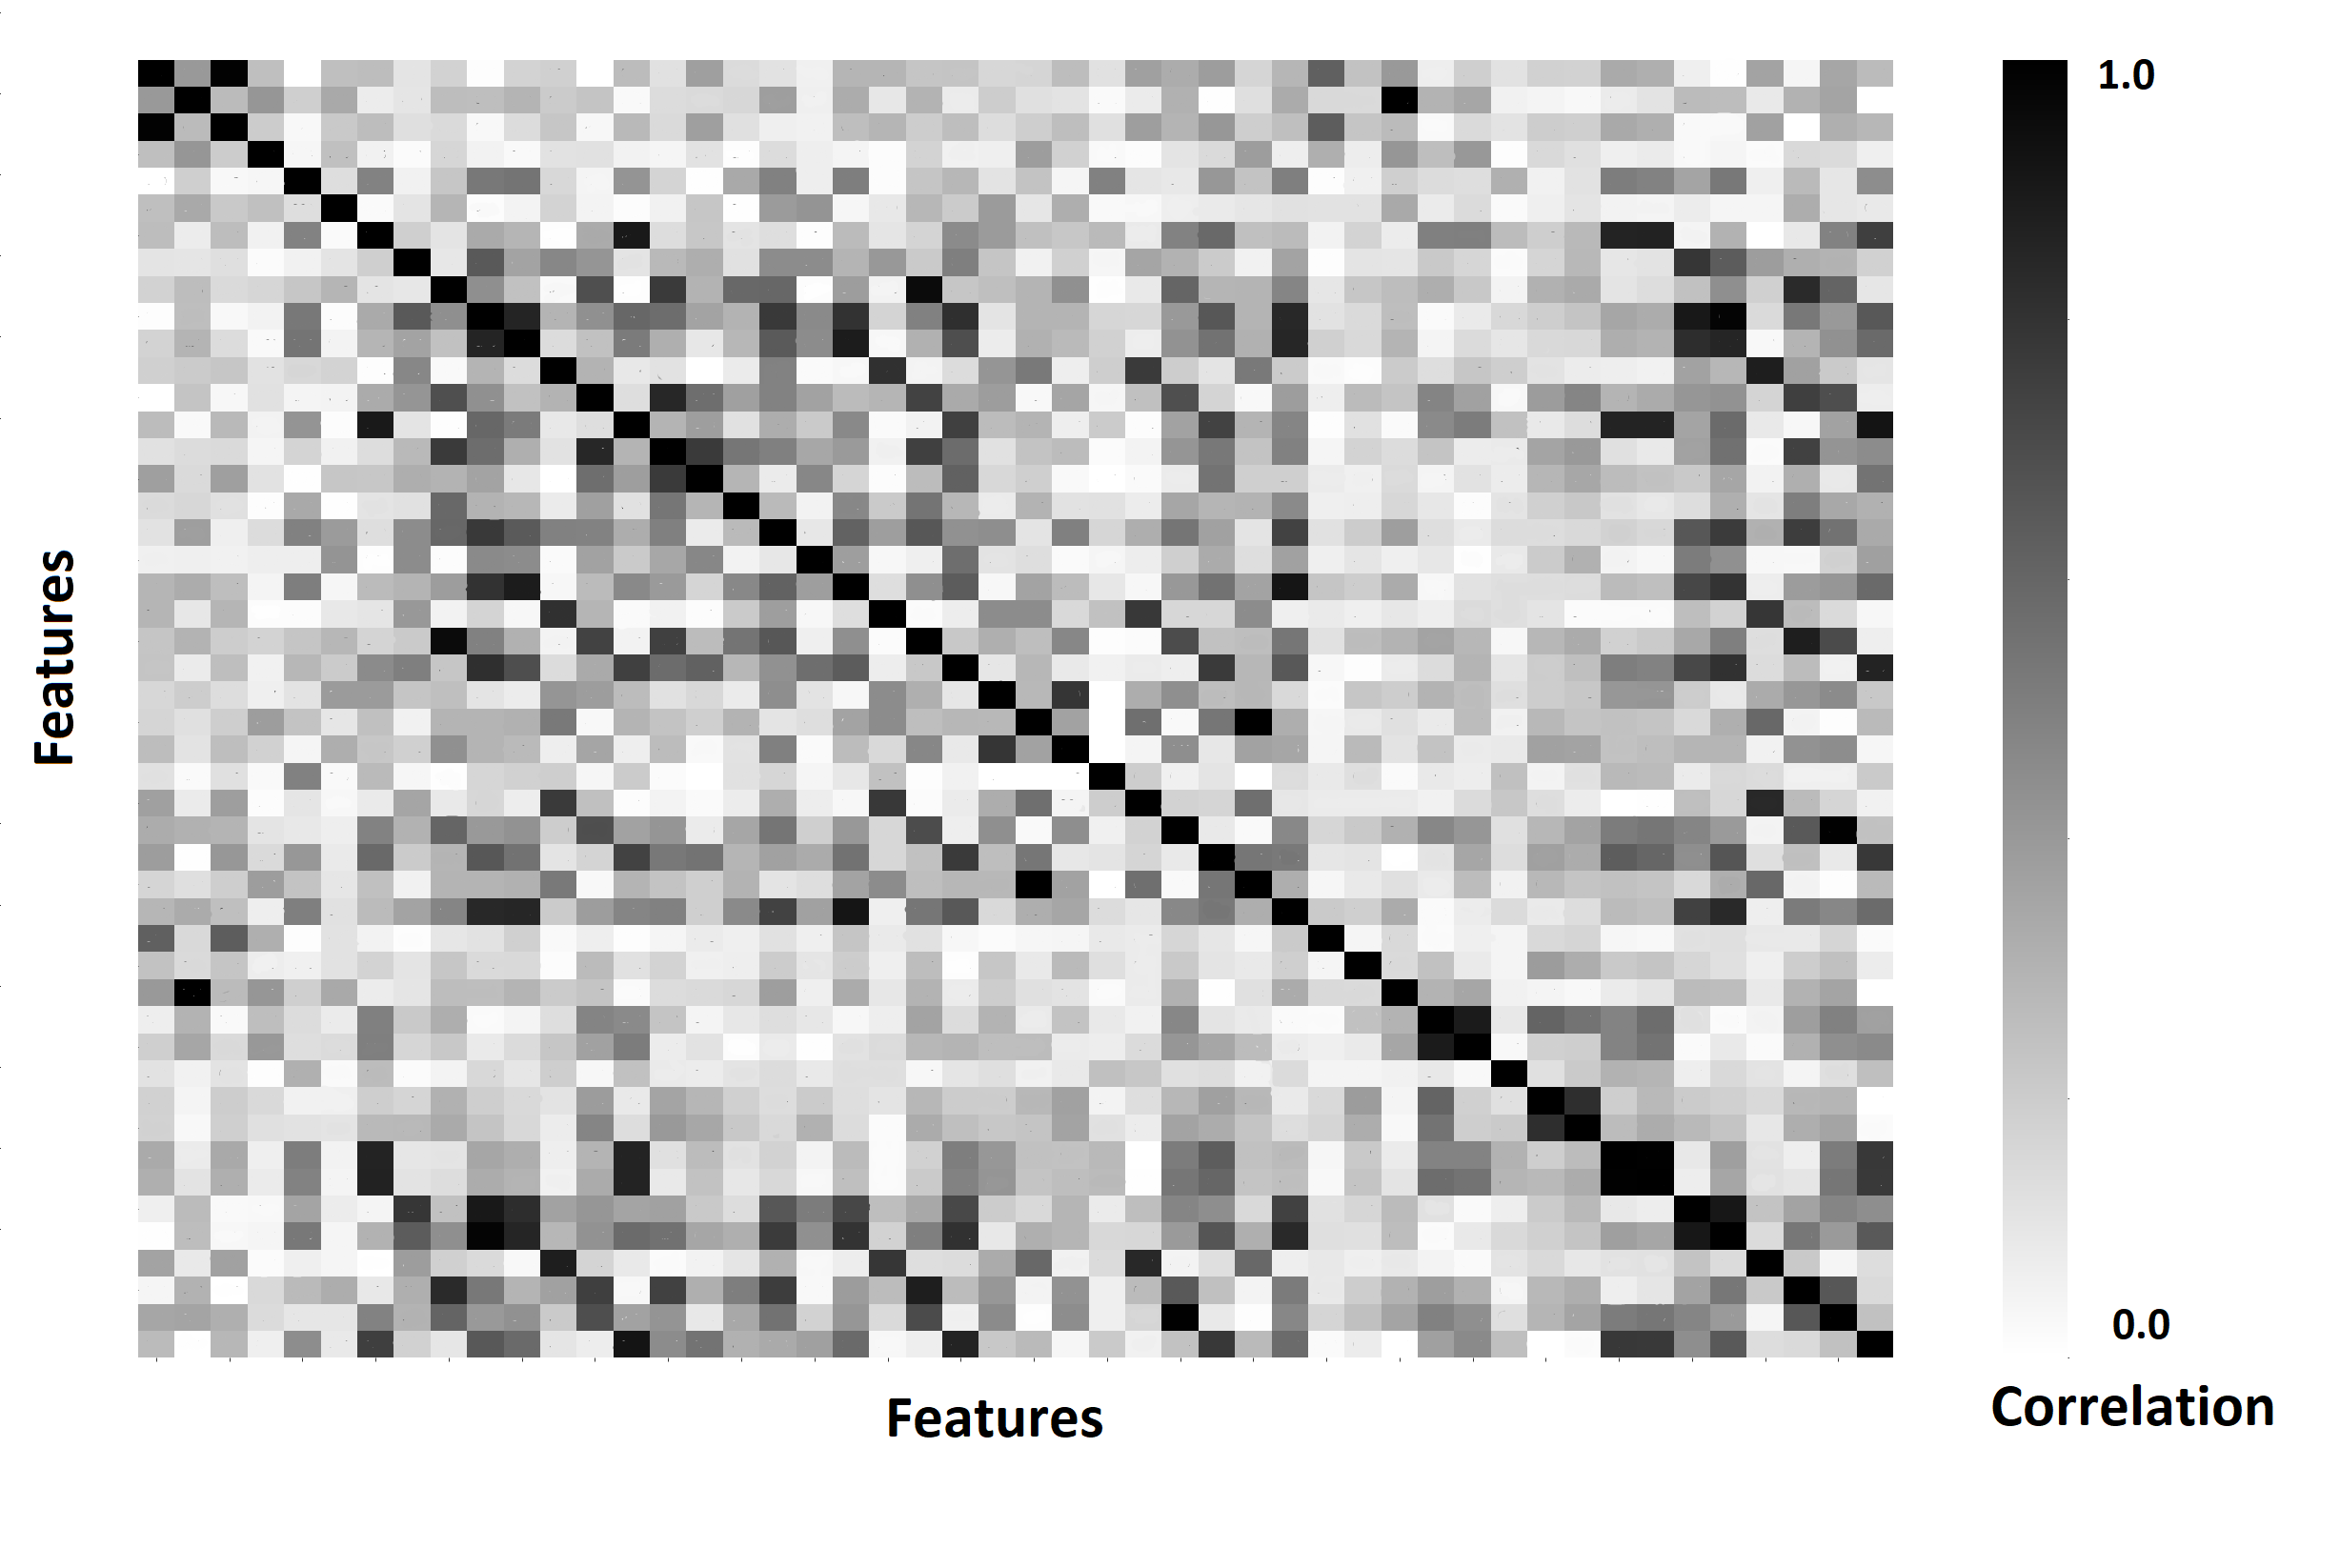
\includegraphics[width=\textwidth, height=5.8cm]{Images/Results/Feature Analysis/feature correlation.png}
    \caption{Correlation before.}
  \end{minipage}
  \hfill
  \begin{minipage}[b]{0.48\textwidth}
    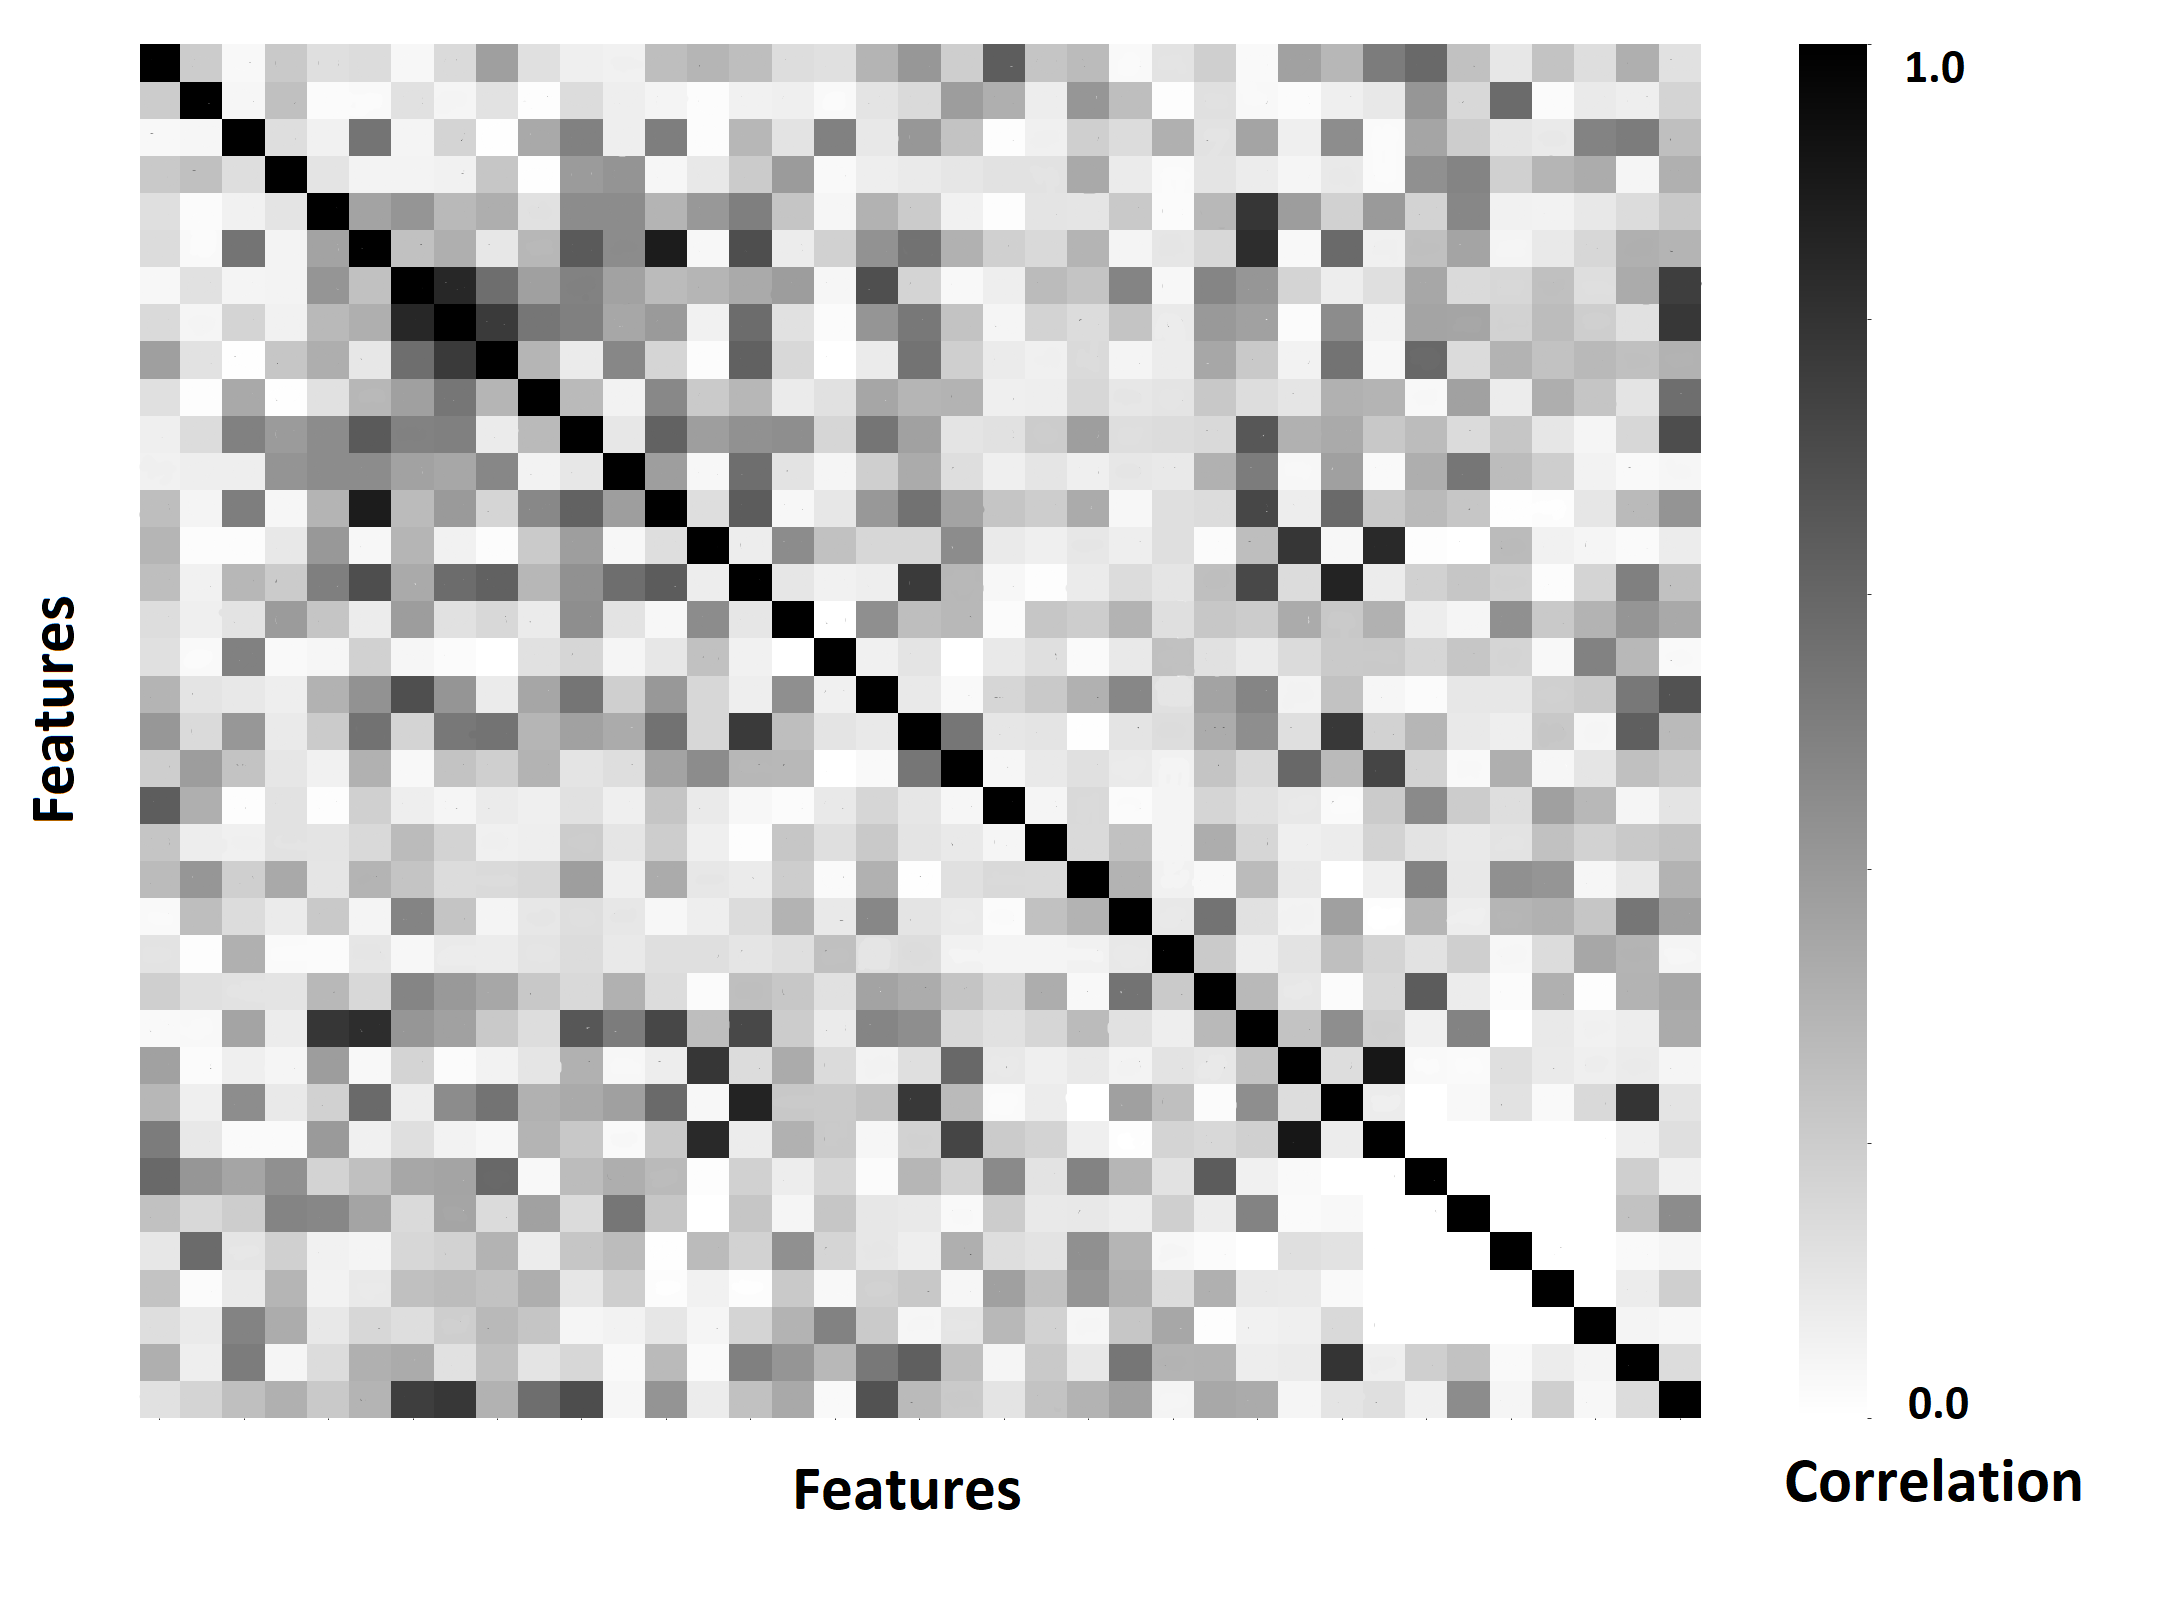
\includegraphics[width=\textwidth]{Images/Results/Feature Analysis/Pearson after.png}
    \caption{Correlation after.}
  \end{minipage}
\end{figure}


\subsubsection{Regressor performance as function of feature number}
Despite the substantial feature reduction, the feature selection algorithm could be used to determine that overfitting was still a problem. Figure 3.11 and Figure 3.12 show the average RMSE for backward feature selection in ridge and Random Forest, respectively.
In these figures, the error drops significantly when most of the relevant features are removed. This is simply due to overfitting, as there are too many features and the observations are not relatively numerous; this does not mean that the features were throwing off the estimation.
\begin{figure}[h!]
    \centering
    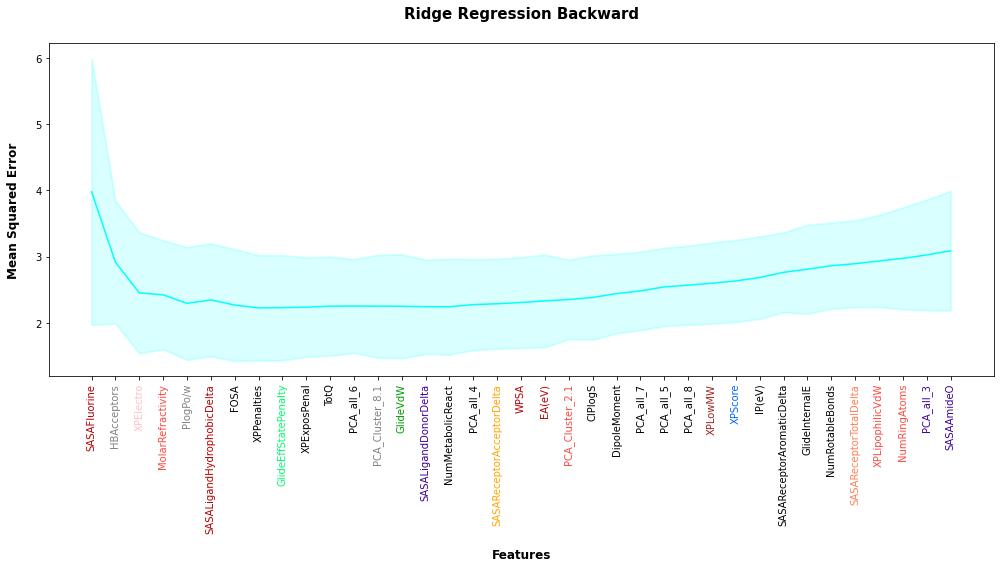
\includegraphics[width=0.8\textwidth]{Images/Results/Ridge Backward.png}
    \caption{Backward feature selection in the ridge regressor.}
\end{figure}
\begin{figure}[h!]
    \centering
    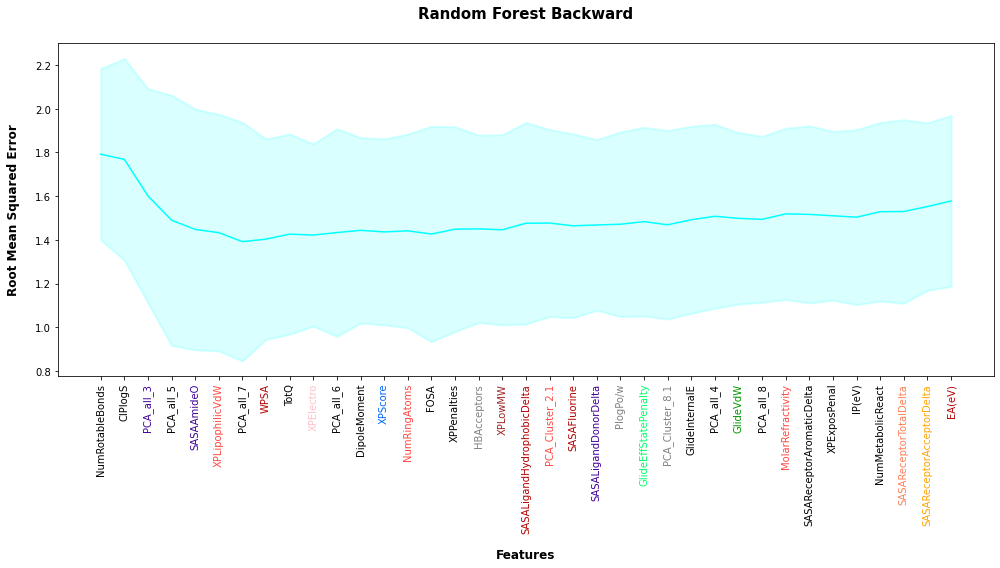
\includegraphics[width=0.8\textwidth]{Images/Results/RF Backward.png}
    \caption{Backward feature selection in the Random Forest regressor.}
\end{figure}

\section{Hyperparameter Optimization}
Once with the feature selection completed, the optimization of hyperparameters of the algorithms to apply (Random Forest and ridge regression) is a very important part. As explained in nested cross-validation, in cases where it wasn't clear which value was the optimal one, a grid search was performed.\\

In the case of \textbf{ridge regression}, the only parameter to optimise was $\alpha$, the regularisation parameter. The learning curve for different values of the regularisation parameter  was plotted (Figure 3.13).

\begin{figure}[h!]
    \centering
    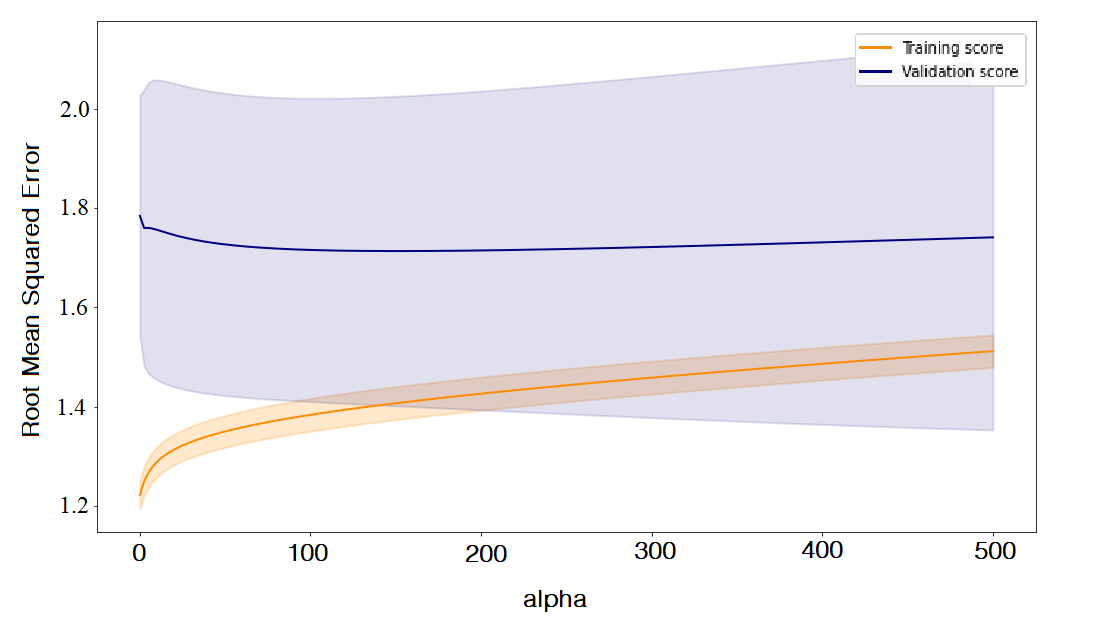
\includegraphics[width=0.8\textwidth]{Images/Results/Hyperparameter/alphalc.png}
    \caption{Learning curves for alpha in ridge regression.}
\end{figure}
It can be seen that the regularization parameter doesn't have a huge impact on the performance of the algorithm, but we can see the a value around 100 might be optimal, which suggests the model is higher variance than it might have seemed.\\

It was decided to do a 250 section grid search from 0 to 125. In the end, the grid search showed inclination towards an unexpectedly small optimal value of $\alpha$ (more in grid search eligibility counts, in the appendix).\\\\

In the case of \textbf{Random Forest}, the hyperparameters which gave out interesting learning curves were firstly, the maximum depth of the decision trees (Figure 3.14); the number of estimators or trees used in the Random Forest; and the maximum number of features taken into account in each tree. This last one was not as important in the end as the distribution was quite homogeneous (more in grid search eligibility counts, in the appendix).\\\\
\begin{figure}
    \centering
    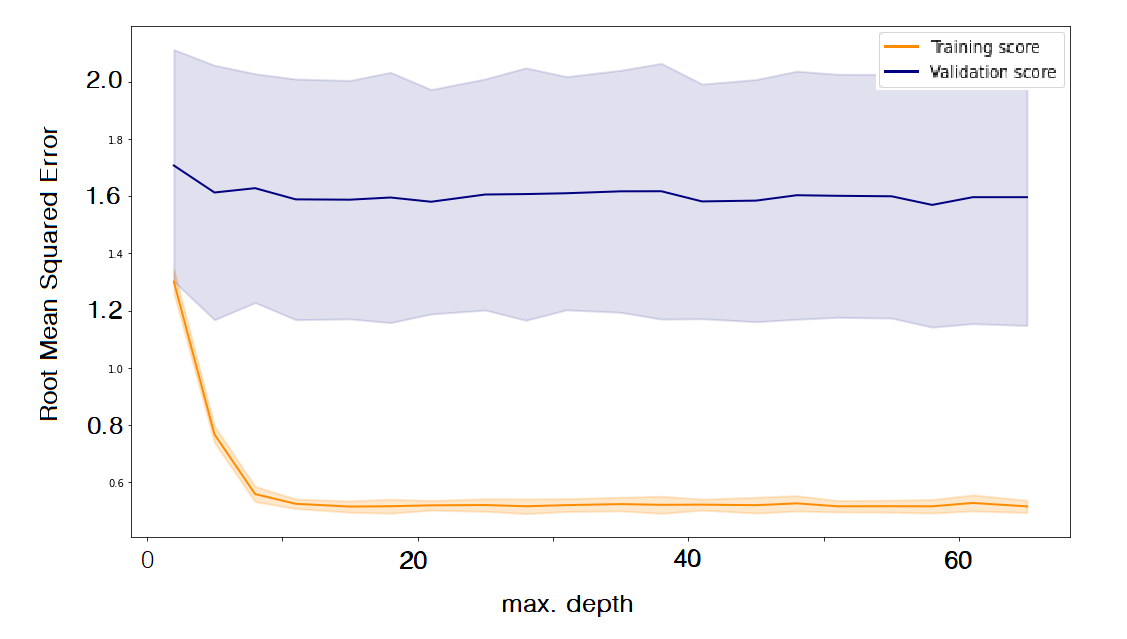
\includegraphics[width=0.8\textwidth]{Images/Results/Hyperparameter/maxdepth.png}
    \caption{Learning curves for maximum depth in Random Forest.}
\end{figure}
Anyhow, a grid search was performed from 1 to 30 in the case of maximum depth; from 25 to 125 with $n$=25 in the number of estimators; and from 0.1 to 1 with $n$=20 in the ratio of maximum features with respect to the total number of features. 


\section{Results}

\subsection{General Evaluation}
After performing nested cross-validation (see Figure 2.11) for each and every regression and correlation metric explained, the obtained values for ridge and Random Forest regression can be visualised in Tables 3.3 and 3.4, respectively.
\begin{table}[h]
\resizebox{\textwidth}{!}{%
\begin{tabular}{l|cccllll|}
\cline{2-8}
                                                   & \multicolumn{1}{l}{\textbf{MAE}}                         & \multicolumn{1}{l}{\textbf{RMSE}}                        & \multicolumn{1}{l}{\textbf{MAPE}}                        & \multicolumn{1}{l}{\textbf{$\rho_p$}}                   & \multicolumn{1}{l}{\textbf{$R^2$}}                       & \multicolumn{1}{l}{\textbf{$\rho_s$}}                    & \multicolumn{1}{l|}{\textbf{$\tau$}}                     \\ \hline
\multicolumn{1}{|l|}{\textbf{Mean}}                & \cellcolor{\color[HTML]{212121} 1.23}      & \cellcolor{\color[HTML]{212121} 2.39}      & \cellcolor{\color[HTML]{212121} 0.085}     & \cellcolor{\color[HTML]{212121} 0.66}     & \cellcolor{\color[HTML]{212121} 0.36}      & \cellcolor{\color[HTML]{212121} 0.61}      & \cellcolor{\color[HTML]{212121} 0.48}      \\
\multicolumn{1}{|l|}{\textbf{95\% CI Mean}}        & \cellcolor{\color[HTML]{212121} 1.18-1.28} & \cellcolor{\color[HTML]{212121} 2.19-2.64} & \cellcolor{\color[HTML]{212121} 0.08-0.09} & \cellcolor{\color[HTML]{212121} 0.61-0.7} & \cellcolor{\color[HTML]{212121} 0.26-0.43} & \cellcolor{\color[HTML]{212121} 0.56-0.66} & \cellcolor{\color[HTML]{212121} 0.43-0.52} \\
\multicolumn{1}{|l|}{\textbf{Standard Error Mean}} & \cellcolor{\color[HTML]{212121} 0.026}     & \cellcolor{\color[HTML]{212121} 0.11}      & \cellcolor{\color[HTML]{212121} 0.0019}    & \cellcolor{\color[HTML]{212121} 0.023}    & \cellcolor{\color[HTML]{212121} 0.044}     & \cellcolor{\color[HTML]{212121} 0.024}     & \cellcolor{\color[HTML]{212121} 0.022}     \\
\multicolumn{1}{|l|}{\textbf{Median}}              & \cellcolor{\color[HTML]{212121} 1.22}      & \cellcolor{\color[HTML]{212121} 2.33}      & \cellcolor{\color[HTML]{212121} 0.086}     & \cellcolor{\color[HTML]{212121} 0.69}     & \cellcolor{\color[HTML]{212121} 0.38}      & \cellcolor{\color[HTML]{212121} 0.64}      & \cellcolor{\color[HTML]{212121} 0.50}      \\
\multicolumn{1}{|l|}{\textbf{Minimum}}             & \cellcolor{\color[HTML]{212121} 0.71}      & \cellcolor{\color[HTML]{212121} 0.81}      & \cellcolor{\color[HTML]{212121} 0.051}     & \cellcolor{\color[HTML]{212121} 0.12}     & \cellcolor{\color[HTML]{212121} -0.68}     & \cellcolor{\color[HTML]{212121} 0.15}      & \cellcolor{\color[HTML]{212121} 0.089}     \\
\multicolumn{1}{|l|}{\textbf{Maximum}}             & 1.71                                                     & 5.00                                                     & 0.13                                                     & 0.90                                                    & 0.79                                                     & 0.89                                                     & 0.77                                                     \\ \hline
\end{tabular}}
\caption{Metrics obtained in the ridge nested CV.}
\end{table}

\begin{table}[h]
\resizebox{\textwidth}{!}{%
\begin{tabular}{l|ccccccc|}
\cline{2-8}
                                                   & \textbf{MAE} & \textbf{RMSE} & \textbf{MAPE} & $\rho_p$  & $R^2$     & $\rho_s$  & $\tau$    \\ \hline
\multicolumn{1}{|l|}{\textbf{Mean}}                & 1.06         & 1.99          & 0.074         & 0.75      & 0.51      & 0.69      & 0.55      \\
\multicolumn{1}{|l|}{\textbf{95\% CI Mean}}        & 1.01-1.12    & 1.75-2.32     & 0.07-0.08     & 0.71-0.78 & 0.43-0.56 & 0.65-0.73 & 0.51-0.58 \\
\multicolumn{1}{|l|}{\textbf{Standard Error Mean}} & 0.030        & 0.15          & 0.0024        & 0.017     & 0.033     & 0.019     & 0.017     \\
\multicolumn{1}{|l|}{\textbf{Median}}              & 1.07         & 1.72          & 0.071         & 0.78      & 0.56      & 0.70      & 0.55      \\
\multicolumn{1}{|l|}{\textbf{Minimum}}             & 0.74         & 0.93          & 0.048         & 0.42      & -0.44     & 0.37      & 0.26      \\
\multicolumn{1}{|l|}{\textbf{Maximum}}             & 1.68         & 5.25          & 0.13         & 0.96      & 0.85      & 0.97      & 0.88      \\ \hline
\end{tabular}}
\caption{Metrics obtained in the Random Forest nested CV.}
\end{table}
Comparing these two tables filled with results, it can be clearly deduced, mainly from the confidence interval section, the results in Random Forest are not only a lot better when it comes to regression error which is lower, but also the correlation metrics seem to be up by a notch. The mean values are also quite better, and the median, which is a good indicator, shows the clear inclination towards improvement.\\\\
\noindent\fbox{%
    \parbox{\textwidth}{%
        It must be said that this enhancement from a simple linear model to a complex non-linear ensemble model such as Random Forest comes at cost in every situation possible, it can be considered universal because of all the distinct metrics used and, therefore, all the scenarios explored. These metrics account for all possible situations, either where there can be outliers in the data or where the data is very trustworthy.
    }%
}
\subsection{Null Hypothesis}
Even after having compared with a ridge regression, the null hypothesis has to be discarded. For this, a so called dummy regressor which estimates the mean of all features' observations and its corresponding RMSE was compared to the actual model and its RMSE. A t-test was performed to check that the obtained performance was statistically significantly different compared to this dummy regressor that always predicts the mean. The null hypothesis is that both models have the same performance (mean RMSE is equal).\\

The t statistic was computed and the p-value was then obtained. This was then compared to the significance $\alpha$, which was chosen to be 0.05. The results obtained were the following:\\
\textbullet\hspace{0.5cm} t statistic: 7.486.\\
\textbullet\hspace{0.5cm} p value: 6.721e-04.\\
Since p \ll $\hspace{0.2cm}\alpha$, the null hypothesis is rejected. The comparison between the RMSEs of the dummy and Random Forest models can be seen in Figure 3.15.
\begin{figure}[h]
    \centering
    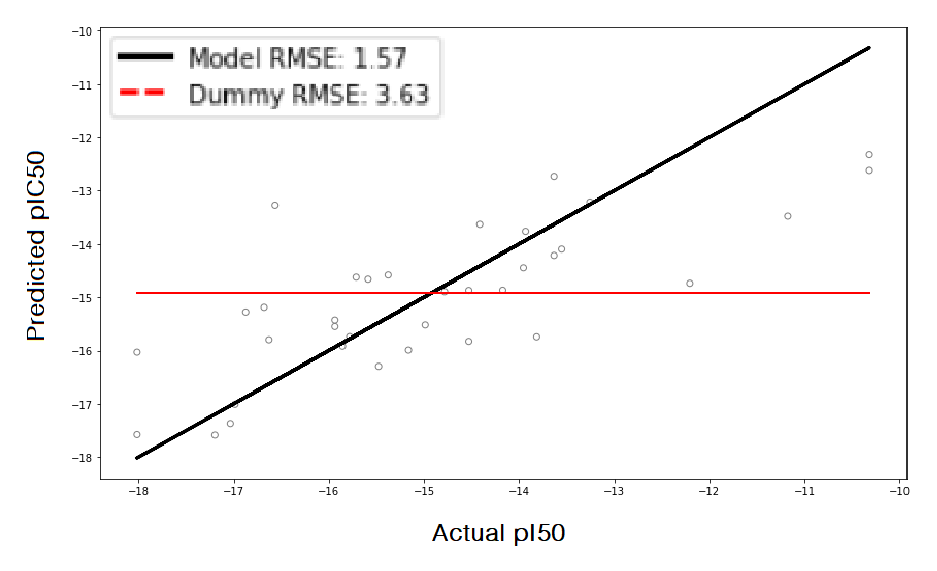
\includegraphics[width=0.6\textwidth]{Images/Results/dummy.png}
    \caption{Performance comparison of the dummy and Random Forest models.}
\end{figure}




\chapter{Discussion}
\hspace{1.5cm}The great thing about machine learning is that there are infinite ways to build a model. Even if an algorithm produces results that are considered very valuable, those positive results can always be revamped in unimaginable ways. In some cases, a common and easy way to improve the model is to collect more data to inflate the dataset, which results in nothing more than a better estimation.\\

These cases, where increasing the size of the dataset improves the model obtained, are the cases where overfitting occurs with a significant amount of data.

\section*{Learning Curves}
As mentioned in the learning curves section (2.3.1), plotting as a function of training set size can be very useful for estimating progress as more observations are added to the data. Ridge regression proved to be underfitting (which was to be expected since it is a simple linear model), but plotting the learning curves for Random Forest yields Figure 4.1. Clearly, overfitting is observed, the training error remains relatively small, while the test error appears unreasonably high.
\begin{figure}
    \centering
    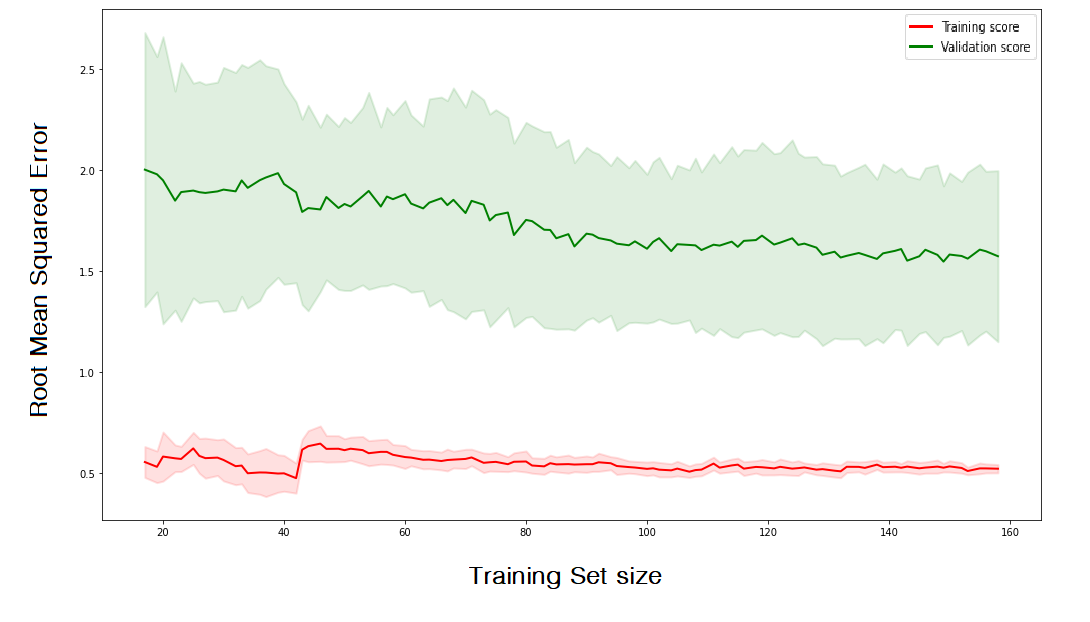
\includegraphics[width=0.6\textwidth]{Images/Discussion/Learningcurve.png}
    \caption{Learning curves for Random Forest with respect to the training set size.}
\end{figure} 

The trends toward lower test error are not clear in the graph, but they are there. Perhaps not in the case where 500 more molecules are added to the dataset, but if the observations of a million molecules, which is not unusual in this respect, were available for training the model, a significant decrease in test error would be seen. Collecting data is usually a rather mechanical process, not very difficult but tedious to do by hand. In this model, the estimation would not have been much better if the size of the dataset had been doubled, but the actual size provides insight into the overfitting that exists and what needs to be done if improvement is intended.\\\\

Sometimes, the opposite action, selectively removing those considered non valuable observations, is another option. More than the non-valuable observations, the clusters where the error is too high can be examined to find the reason. This can be taken further using cluster error analysis.
\section*{Cluster Based Error Analysis}
With respect to what should the observations be clustered? Descriptors can be chosen, or even the response feature. Another valuable option is using the molecular fingerprints as the criterion.
\subsection*{Molecular Fingerprints}
To calculate fingerprints for a series of molecules, it is necessary for the dataframe to have a column describing the \textbf{SMILES} chains of the molecules. SMILES chains describe the structure of a molecule in a simplified form, with all its atoms (except for hydrogen) and the types of bonds between them. An example would be, glucose: C([C@@H]1[C@H]([C@@H]([C@H](C(O1)O)O)O)O)O . But how to arrive at clusters starting with these identifiers? From these SMILES chains, a conventional 1024-bit fingerprint is created for each molecule. This fingerprint can be represented as a 1024-dimensional vector with ones and zeroes. Each 1 would refer to the existence of a substructure determined in the algorithm. This vector is now viable to be a clustering criterion.\\

K-fold clustering was carried on, and k=11 was used. In Figure 4.2 are 8 of the 22 molecules in the first cluster where conformation similarities can be clearly spotted.
\begin{figure}[h!]
    \centering
    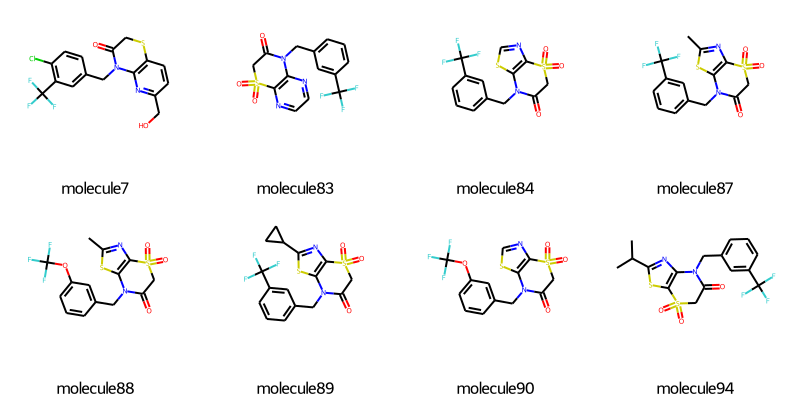
\includegraphics[width=0.7\textwidth]{Images/Discussion/clusterfinger.png}
    \caption{Molecules corresponding to Cluster 1 after carrying out k-fold clustering in molecular fingerprints.}
\end{figure}

The errors in each cluster vary as it can be perceived in Figure 4.3.
\begin{figure}[h]
    \centering
    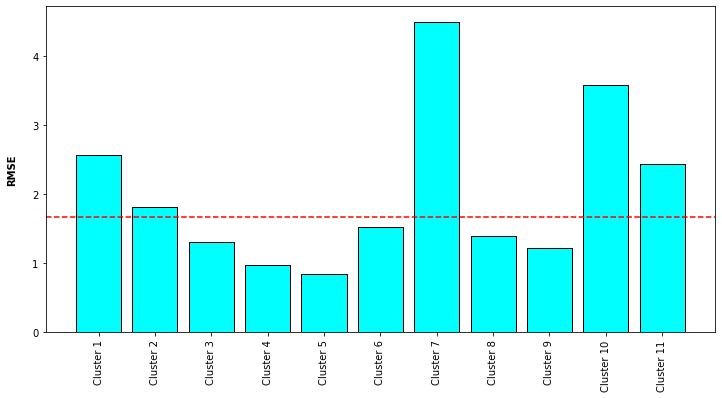
\includegraphics[width=0.8\textwidth]{Images/Discussion/clustererror.png}
    \caption{Error found in each cluster in Random Forest.}
\end{figure}


\section*{Metaregressors}
When it comes to the algorithm itself and the choice of making to solve for this problem, even if Random Forest was a good choice, there is no perfect regressor, and the option can be improved to get even better results.\\

The better half of this problem resides in metaregressors, which are ensembles of algorithms such as Random Forest and Support Vector Machines. These metaregressors are designed to optimize even further in expense of computation, they are very promising.\\\\\\\\\\\\\\



\section*{Conclusion}
In conclusion, a larger hereness of molecule data or the creation of a database with a large number of molecules could significantly improve the model; and not only that, the application of a metaregressor combined with this could potentially refine a huge lot the results obtained. Even with all this said, the Random Forest algorithm performed very well and deserves the credit granted.

\bibliographystyle{plain}
\bibliography{bibliography}

\pagestyle{plain}




\end{document}


\end{document}